%%%%%%%%%%%%%%%%%% Environment
\documentclass[12pt]{article}
\usepackage[utf8]{inputenc}
%\documentclass{article}
%\usepackage{beamerarticle}

%%%%%%%%%%%%%%%%%% Basic Packages
\usepackage{amsbsy}
\usepackage{amstext}
\usepackage{amsfonts}
\usepackage{amssymb}
\usepackage{amsthm}
\usepackage{amsmath}
\usepackage{bbm}
\usepackage{color}
\usepackage{arydshln}
\usepackage{multirow}
\usepackage{changepage}
\usepackage{threeparttable,booktabs}
\usepackage{enumitem}
\usepackage{subfigure}
\usepackage{natbib}

%\usepackage{natbib}
%\bibliographystyle{abbrvnat}
%\setcitestyle{authoryear,open={((},close={))}}

%%%%%%%%%%%%%%%%%% Style
\usepackage[margin=1in]{geometry}%
\usepackage{setspace}
\doublespacing
%\usepackage{setspace}
%\setstretch{1.618}
%%%%%%%%%%%%%%%%%% Fonts and Graphics
\usepackage[cjk]{kotex} %Korean TeX
\usepackage[pdftex]{graphicx}

%%%%%%%%%%%%%%%%%% Theorem
\newtheorem{Theorem}{Theorem}
\newtheorem{Lemma}{Lemma}
\newtheorem{assumption}{Assumption}
\newtheorem{prop}{Proposition}
\newtheorem{corollary}{Corollary}
\newcommand{\ju}{\textcolor{cyan}}
\newcommand{\yj}{\textcolor{magenta}}
\usepackage{apptools}
\AtAppendix{\counterwithin{Lemma}{section}}
\AtAppendix{\counterwithin{table}{section}}
\AtAppendix{\counterwithin{figure}{section}}

%%%%%%%%%%%%%%%%%% Bibliography and Appendices
%\usepackage[natbibapa]{apacite} % Including URLs in bibliography
\usepackage{natbib}
\usepackage[hyphens]{url} % Including URLs in bibliography
%\usepackage[toc,page,title]{appendix} % Extra control of appendices
\usepackage[titletoc,toc,title]{appendix}
\usepackage{chngcntr}

%%%%%%%%%%%%%%%%%% Beginning of the Manuscript
\begin{document}

\begin{center}\textbf{\Large Online Supplementary Materials for }\end{center}
\begin{center}{\LARGE Sharing Economy in the Cloud: Pricing Schemes for Peer-to-Peer Storage Platforms}\end{center}

\appendix
\renewcommand{\thesection}{\Alph{section}}

\section{Algorithmic Backgrounds}\label{app:algorithm}
In general, P2P storage platforms utilize erasure coding in their redundancy algorithms to ensure high levels of file availability. Under a $k$-of-$m$ erasure coding scheme, the P2P storage platform divides a renter's original file into $k$ shards and re-codes them into $m$ encrypted fragments ($m > k$) \citep{weatherspoon2002erasure, wilkinson2016storj}. Then, the platform assigns each of $m$ fragments to $m$ independent providers who have made a contract with the focal renter. Notably, any $k$ of $m$ fragments can reconstruct the file under this redundancy algorithm. Therefore, the platform can retrieve the file when any $k$ providers are connected to the network at the same time. As such, the main advantage of erasure coding is that it can achieve high reliability with a low redundancy rate $\theta(=\frac{m}{k})$ \citep{weatherspoon2002erasure}. We can easily estimate the reliability of the P2P storage networks as follows. Given the redundancy parameters $k$, $n$ and the required uptime $t$, the failure probability is calculated as:

\begin{equation*}
\begin{aligned}
F(t; m, k) = \sum_{j=0}^{k-1} {m \choose j}t^j (1-t)^{m-j}
\end{aligned}
\end{equation*}

From the equation above, we obtain the following relationships between the failure probability, the redundancy parameters and the required uptime:

\begin{Lemma}\label{lem:uptime}
i) $F(t; m, k)$ is decreasing in $t$ for fixed $m$ and $k$,\\
ii) $F(t; m, k)$ is decreasing in $m$ for fixed $t$ and $k$.
\end{Lemma}

Lemma \ref{lem:uptime} provides insight into how each parameter affects the failure probability. First, the failure probability decreases when the platform requires a higher uptime to the provider, indicating that the platform can enhance the reliability while maintaining the same redundancy rate by imposing higher responsibility on the provider. Second, if the platform assigns the file fragments to a larger number of providers, the failure probability decreases. It suggests that the platform can improve the file availability by increasing the number of providers instead of imposing higher responsibility on each provider.

Table \ref{tbl:redundancy_1} presents the calculated failure probability under the given redundancy $\theta = 3$. We observe that the platform can improve its system reliability even when it maintains the same redundancy $\theta$ and the same required uptime $t$. For instance, for $\theta=3$ and $t=0.75$, the failure probability is 1.15e-04 when the platform sets $k=5$ and $m=15$. Notably, the platform can reduce the failure probability by about 400 times (from 1.15e-04 to 2.82e-07) by dividing the files into twice more fragments ($k=10$ and $m=30$) without altering $\theta$ and $t$. Moreover, we see that a small increase in the required uptime can dramatically reduce the failure probability. For example, when all other things are same, raising the required $t$ by 20\% (from 0.75 to 0.90) under $k=10$ and $n=30$ decreases the failure by 48.6 million times (from 2.82e-07 to 5.80e-15).

\begin{table}[h]
\textbf{\caption{An Example of Redundancy Algorithm and Failure Probability ($\theta=3$)\label{tbl:redundancy_1}}}
\begin{center}
\begin{tabular}{cccc}
 $m$ & $k$ & $t$ & $F(t; m, k)$\\\hline
15 & 5 & 0.5 & 5.92e-02\\
15 & 5 & 0.75 & 1.15e-04\\
15 & 5 & 0.9 & 9.30e-09\\
15 & 5 & 0.99 & 1.32e-19\\
30 & 10 & 0.5 & 2.14e-02\\
30 & 10 & 0.75 & 2.82e-07\\
30 & 10 & 0.9 & 5.80e-15\\
30 & 10 & 0.99 & 1.31e-35\\
\end{tabular}
\end{center}
\end{table}

In addition to erasure coding, P2P storage platforms are taking several measures to prevent the strikingly adverse effect of file transfer failure. For instance, P2P storage platforms usually require providers to meet the minimum available storage space, computing power of processors, and bandwidth speed. Also, they mandate the uptime level in various ways. Sia expects providers to maintain 95–98\% uptime to achieve 99.9999\% accessibility of stored files. If a provider in the Sia network does not maintain 95\% uptime (or 36 hours off in a month), he will lose his collateral for active contracts. Storj requires a more demanding uptime requirement that requires providers to maintain 99.3\% uptime (or 5 hours of maximum downtime per month). Filecoin assesses miners in the cryptocurrency network and penalizes storage providers using the miners' collateral if they do not perform the proof-of-spacetime. Hypothetically, Sia and Storj are expected to achieve the very low failure probability as 2.52e-29 and 2.11e-91 based on their algorithm parameters ($k, m, t$) as $(10, 30, 0.98)$ and $(29, 80, 0.993)$, respectively.\footnote{The relevant information was retrieved from the following sources: 1) Storj's redundancy parameters (https://docs.storj.io/concepts/overview), 2) Storj's required uptime (https://www.storj.io/node-operator-terms-conditions), 3) Sia's redundancy parameters (https://support.sia.tech/renting/is-my-data-secure\#security), 4) Sia's required uptime (https://support.sia.tech/hosting/about-hosting-on-sia).} According to Storj, the Tardigrade platform---Storj's main service---demonstrated 99.96\% availability in practice.\footnote{Please refer to the following webpage for further details: https://www.storj.io/blog/announcing-pioneer-2-and-tardigrade-io-pricing.}

If we assume that the target failure probability $\bar{p}$ is close to zero, i.e., $\bar{p} \approx 0$, the platform's redundancy parameters and the required uptime satisfy the following equation:
\begin{equation*}
\begin{aligned}
F(t; m, k) = \sum_{j=0}^{k-1} {m \choose j}t^j (1-t)^{m-j} \le \bar{p}.
\end{aligned}
\end{equation*}
As shown in Lemma \ref{lem:uptime}, the platform achieves its target failure probability by requiring a high uptime $t$ or adopting a high redundancy rate $\theta$. Table \ref{tbl:redundancy_2} presents the calculated pair of the redundancy rate and the required uptime for $k=10$ and the target probability $\bar{p} = 10e-10$. Figure \ref{fig:redundancy} visualizes this relationship. When a redundancy rate is low, increasing $\theta$ does not significantly decrease the required uptime. For instance, when $\theta$ increases from 1 to 1.5, the required $t$ decreases by only 0.005. In contrast, when we compare $\theta = 3$ and $\theta = 3.5$, the required uptime decreased by (from 0.836 to 0.776).

\begin{table}[h]
\textbf{\caption{An Example of Redundancy Rate and Uptime ($k=10$, $\bar{p} = 10^{-10}$)\label{tbl:redundancy_2}}}
\begin{center}
\begin{tabular}{cccccc}
 $\theta$ &$t$&$\theta$ & $t$&$\theta$&$t$\\\hline
$\le$1.2 & 1 & 2.0 & 0.957 & 2.8 & 0.861\\
1.3 & 0.999 & 2.1 & 0.947 & 2.9 & 0.849\\
1.4 & 0.998 & 2.2 & 0.935 & 3.0 & 0.836\\
1.5 & 0.995 & 2.3 & 0.924 & 3.1 & 0.824\\
1.6 & 0.990 & 2.4 & 0.911 & 3.2 & 0.812\\
1.7 & 0.984 & 2.5 & 0.899 & 3.3 & 0.800\\
1.8 & 0.976 & 2.6 & 0.886 & 3.4 & 0.788\\
1.9 & 0.967 & 2.7 & 0.874 & 3.5 & 0.776\\
\end{tabular}
\end{center}
\end{table}

\begin{figure}[ht!]
\centering
\includegraphics[width=10cm]{figure_3rd_final/uptime_fig.jpg} 
\textbf{\caption{Redundancy Rate and Required Uptime ($k=10$, $\bar{p} = 10^{-10}$)\label{fig:redundancy}}}
\end{figure}

\clearpage

\section{Proof}\label{app:proof}
% Before we proceed the proofs of the main results, we analyze providers' participation decision to the P2P storage service and derive the results in the lemma below.

\paragraph{Proof of Lemma 1}
\begin{proof}
Provider \textit{j}'s cost increases in $\rho_j$. Thus, if $\pi|_{\rho_j = 1} \ge 0$, all providers are profitable (i.e., $\rho_m = 1$). Otherwise, if $\pi|_{\rho_j= 1} <0$, there exists $\rho_m < 1$ that satisfies $\pi|_{\rho_j = \rho_m} = 0$. Also, if $\omega_s \le \theta \upsilon_s $, all providers' utilization becomes $1$. In contrast, when $\theta \upsilon_s < \omega_s $, all providers' utilization is strictly lower than $1$. We thus consider the following cases:
\begin{table}[h]
\begin{center}
\begin{tabular}{c|cc}
&$\pi|_{\rho_j = 1} \ge 0$ & $\pi|_{\rho_j = 1} < 0$\\\hline 
$\omega_s \le \theta \upsilon_s$ & $\rho_m = 1$, $\hat{\omega}_s=1 $ & $\rho_m < 1$, $\hat{\omega}_s=1 $\\
$\theta \upsilon_s < \omega_s$& $\rho_m = 1$, $\hat{\omega}_s<1 $ & $\rho_m < 1$, $\hat{\omega}_s<1 $\\
\end{tabular}
\end{center}
\end{table}

\noindent \textbf{A. Analysis of Cases and Sub-conditions}\\
We analyze the four cases as follows. First, we derive the outcome of each case and its sub-conditions. Then, we assess the feasibility of these outcomes.\\

\noindent \textbf{\textit{Case A1:}} $\pi|_{\rho_j =1} \ge 0$ and $\omega_s \le \theta \upsilon_s$.

\noindent This condition leads to $\rho_m = 1$ and $\hat{\omega}_s = 1$. For each of the two sub-conditions, we obtain the followings:

\textit{\underline{Sub-condition A1-i:}} $\pi|_{\rho_j = 1} \ge 0$:
\begin{equation*}
\begin{aligned}
&\pi|_{\rho_j = 1} \ge 0 \Leftrightarrow \alpha p_s + \alpha p_b \frac{\upsilon_{bp}}{\theta \upsilon_s} - \frac{\xi \upsilon_b}{\theta \upsilon_s} \ge 0 \\
&\Leftrightarrow \frac{\xi \upsilon_b}{\theta \upsilon_s} \le \alpha p_s + \alpha p_b \frac{\upsilon_{bp}}{\theta \upsilon_s} \Leftrightarrow g_1 \le \tilde{\pi}, 
\end{aligned}
\end{equation*}

\textit{\underline{Sub-condition A1-ii:}} $\omega_s \le \theta \upsilon_s$:
\begin{equation*}
\begin{aligned}
&\omega_s \le \theta \upsilon_s \Leftrightarrow n_p \le \theta \upsilon_s.
\end{aligned}
\end{equation*}

As a result, we obtain $(\rho_m, \hat{\omega}_s) = (1, 1)$.\\

\noindent \textbf{\textit{Case A2:}} $\pi|_{\rho_j =1} <0$ and $\omega_s \le \theta \upsilon_s$.\\
\noindent In this condition, $\rho_m <1$ and $\hat{\omega}_s = 1$. Then, the sub-conditions lead to the following results:

\textit{\underline{Sub-condition A2-i:}} $\pi|_{\rho_j = \rho_m} = 0$ where $\rho_m < 1$: 
\begin{equation*}
\begin{aligned}
&\pi|_{\rho_j = \rho_m} = 0 \Leftrightarrow \alpha p_s + \alpha p_b \frac{\upsilon_{bp}}{\theta \upsilon_s} - \rho_m \frac{\xi \upsilon_b}{\theta \upsilon_s} = 0 \Leftrightarrow \rho_m = \frac{\alpha p_s + \alpha p_b \frac{\upsilon_{bp}}{\theta \upsilon_s}}{\frac{\xi \upsilon_b}{\theta \upsilon_s}} \\
&\Rightarrow \rho_m < 1 \Leftrightarrow \frac{\alpha p_s + \alpha p_b \frac{\upsilon_{bp}}{\theta \upsilon_s}}{\frac{\xi \upsilon_b}{\theta \upsilon_s}} < 1 \Leftrightarrow \tilde{\pi}<g_1,
\end{aligned}
\end{equation*} 

\textit{\underline{Sub-condition A2-ii:}} $\omega_s \le \theta \upsilon_s$:
\begin{equation*}
\begin{aligned}
&\omega_s \le \theta \upsilon_s \Leftrightarrow n_p \rho_m \le \theta \upsilon_s \Leftrightarrow n_p \frac{\alpha p_s + \alpha p_b \frac{\upsilon_{bp}}{\theta \upsilon_s}}{\frac{\xi \upsilon_b}{\theta \upsilon_s}} \le \theta \upsilon_s\\
&\Leftrightarrow \alpha p_s + \alpha p_b \frac{\upsilon_{bp}}{\theta \upsilon_s}  \le \frac{\xi \upsilon_b}{n_p} \Leftrightarrow \tilde{\pi} \le g_2. 
\end{aligned}
\end{equation*}

It follows that $(\rho_m, \hat{\omega}_s) = (\frac{\tilde{\pi}}{g_1}, 1)$.\\

\noindent \textbf{\textit{Case A3:}} $\pi|_{\rho_j =1} \ge 0$ and $\theta \upsilon_s < \omega_s $.\\
This condition results in $\rho_m = 1$ and $\hat{\omega}_s = \frac{\theta \upsilon_s}{\omega_s}$. The two sub-conditions lead to the followings:

\textit{\underline{Sub-condition A3-i:}} $\pi|_{\rho_j = 1} \ge 0$:
\begin{equation*}
\begin{aligned}
&0 \le \pi|_{\rho_j = 1} \Leftrightarrow 0 \le \alpha p_s + \alpha p_b \frac{\upsilon_{bp}}{\theta \upsilon_s} - \frac{\xi \upsilon_b}{\theta \upsilon_s}\\
&\Leftrightarrow \frac{\xi \upsilon_b}{\theta \upsilon_s} \le \alpha p_s + \alpha p_b \frac{\upsilon_{bp}}{\theta \upsilon_s} \Leftrightarrow g_1 \le \tilde{\pi}, 
\end{aligned}
\end{equation*}

\textit{\underline{Sub-condition A3-ii:}} $ \theta \upsilon_s < \omega_s$:
\begin{equation*}
\begin{aligned}
&\theta \upsilon_s < \omega_s \Leftrightarrow \theta \upsilon_s < n_p.
\end{aligned}
\end{equation*}

Then, $ (\rho_m, \hat{\omega}_s) = (1, \frac{\theta \upsilon_s}{n_p})$.\\

\noindent \textbf{\textit{Case A4:}} $\pi|_{\rho_j =1} <0$ and $\theta \upsilon_s < \omega_s $.\\
This condition leads to $\rho_m <1$ and $\hat{\omega}_s = \frac{\theta \upsilon_s}{\omega_s}$. For the two sub-conditions, we obtain the followings:

\textit{\underline{Sub-condition A4-i:}} $\pi|_{\rho_j = \rho_m} = 0$ where $\rho_m < 1$:
\begin{equation*}
\begin{aligned}
&\pi|_{\rho_j = \rho_m} = 0 \Leftrightarrow \alpha p_s + \alpha p_b \frac{\upsilon_{bp}}{\theta \upsilon_s} - \rho_m \frac{\xi \upsilon_b}{\theta \upsilon_s} = 0 \Leftrightarrow \rho_m = \frac{\alpha p_s + \alpha p_b \frac{\upsilon_{bp}}{\theta \upsilon_s}}{\frac{\xi \upsilon_b}{\theta \upsilon_s}} \\
&\Rightarrow \rho_m < 1 \Leftrightarrow \frac{\alpha p_s + \alpha p_b \frac{\upsilon_{bp}}{\theta \upsilon_s}}{\frac{\xi \upsilon_b}{\theta \upsilon_s}} < 1 \Leftrightarrow \tilde{\pi} < g_1,
\end{aligned}
\end{equation*}

\textit{\underline{Sub-condition A4-ii:}} $\theta \upsilon_s < \omega_s$: 
\begin{equation*}
\begin{aligned}
&\theta \upsilon_s < \omega_s \Leftrightarrow \theta \upsilon_s < n_p \rho_m \Leftrightarrow \theta \upsilon_s < n_p \frac{\alpha p_s + \alpha p_b \frac{\upsilon_{bp}}{\theta \upsilon_s}}{\frac{\xi \upsilon_b}{\theta \upsilon_s}} \\
&\Leftrightarrow   \frac{\xi \upsilon_b}{n_p}  <   \alpha p_s + \alpha p_b \frac{\upsilon_{bp}}{\theta \upsilon_s} \Leftrightarrow g_2 < \tilde{\pi}.   
\end{aligned}
\end{equation*}

Therefore, we observe that $ (\rho_m, \hat{\omega}_s) = (\frac{\tilde{\pi}}{g_1}, \frac{g_2}{\tilde{\pi}} )$. \\

\noindent \textbf{B. Feasibility Analysis}\\
For the results obtained above, we analyze the feasibility of each case. Since $\theta \upsilon \lessgtr n_p \Leftrightarrow g_2 \lessgtr g_1$ holds, we consider the following cases:\\

\noindent \textbf{\textit{Case B1:}} $\theta \upsilon_s \le n_p$.\\
This case implies $g_2 \le g_1$. By using this property, we analyze the feasible region for each of the cases in part A:

\textbf{\textit{Case A1:}} infeasible,

\textbf{\textit{Case A2:}} when $\tilde{\pi} \le g_2$, $(\rho_m, \hat{\omega}_s) = (\frac{\tilde{\pi}}{g_1}, 1)$,

\textbf{\textit{Case A3:}} when $g_1 \le \tilde{\pi}$, $(\rho_m, \hat{\omega}_s) = (1, \frac{\theta \upsilon_s}{n_p})$,

\textbf{\textit{Case A4:}} when $g_2 < \tilde{\pi} < g_1$, $(\rho_m, \hat{\omega}_s) = (\frac{\tilde{\pi}}{g_1}, \frac{g_2}{\tilde{\pi}})$.

Combining these feasible regions and the continuity of $(\rho_m, \hat{\omega}_s)$ across the cases, we obtain the results for $\theta \upsilon_s \le n_p$, as shown in Lemma 1.\\

\noindent \textbf{\textit{Case B2:}} $\theta \upsilon_s \ge n_p$.
In this case, we see $g_2 \ge g_1$. For each case in the part A, we obtain the feasible region as follows:

\textbf{\textit{Case A1:}} when $g_1 \le \tilde{\pi}$, $(\rho_m, \hat{\omega}_s) = (1, 1)$,

\textbf{\textit{Case A2:}} when $\tilde{\pi} < g_1$, $(\rho_m, \hat{\omega}_s) = (\frac{\tilde{\pi}}{g_1}, 1)$,

\textbf{\textit{Case A3:}} infeasible,

\textbf{\textit{Case A4:}} infeasible.

Incorporating these feasible regions and the continuity of $(\rho_m, \hat{\omega}_s)$, we obtain the results for $n_p \le \theta \upsilon_s$ in Lemma 1.
\end{proof}


\paragraph{Proof of Lemma 2}
\begin{proof}
We derive the profit-maximizing service fees for each pricing scheme. In doing so, we separate the hybrid pricing into two cases based on whether the free bandwidth allowance exceeds the minimum usage level $\lambda_0$.\\  

\noindent \textbf{\textit{Case 1: The Two-part Tariff.}}\\
We consider the two sub-cases according to the value of the storage service fee $p_s$ as follows:

\textit{\underline{Sub-case 1-i:}} $0 \le p_s \le \frac{\lambda_0 - \lambda_0 p_b}{\theta}$.

Regarding renters willing to adopt the platform, the total storage volume $\upsilon_s$ and the total paid bandwidth volume $\upsilon_{bp}$ are derived as follows:
\begin{equation*}
\begin{aligned}
&\upsilon_s = n_r \int_{\lambda_0}^{\infty}(1-\frac{\theta p_s}{\lambda} - p_b) f(\lambda) d \lambda = n_r(1-\frac{2\theta p_s}{3\lambda_0} - p_b),\\
&\upsilon_{bp} = n_r \int_{\lambda_0}^{\infty}\lambda (1-\frac{\theta p_s}{\lambda} - p_b) f(\lambda) d \lambda  = n_r\left[-\theta p_s + 2\lambda_0 (1-p_b) \right].
\end{aligned}
\end{equation*}

Using the derived $\theta \upsilon_s$ and $\upsilon_{bp}$, we can rewrite the platform's objective function as:
\begin{equation*}
\max_{p_s, p_b}\Pi(p_s, p_b) = (1-\alpha) \theta n_r \left( - \frac{2\theta}{3\lambda_0} p_s^2 - 2 p_s p_b - \frac{2\lambda_0}{\theta} p_b^2 + p_s + \frac{2\lambda_0}{\theta} p_b\right).
\end{equation*}

We verify the second-order condition by analyzing the Hessian matrix of that profit function
\begin{equation*}
H=\begin{bmatrix}
-\frac{4(1-\alpha) \theta^2 n_r}{3\lambda_0} & -2(1-\alpha) \theta n_r\\
-2(1-\alpha) \theta n_r & -4 (1-\alpha) \lambda_0 n_r
\end{bmatrix}.
\end{equation*}

We observe that the first-order leading principal minor is negative and the second-order leading principal minor is $det(H) = \frac{4}{3}(1-\alpha)^2 \theta^2 n_r^2 >0$. Therefore, $H$ is negative-definite. Hence, the second-order condition is satisfied, and this profit function has the global maximum. Based on these results, we obtain the optimal service fees as:\\
\begin{equation*}
\left(p_s^T, p_b^T\right) = \left(0, \frac{1}{2}\right).
\end{equation*}

\textit{\underline{Sub-case 1-ii:}} $p_s \ge \frac{\lambda_0 - \lambda_0 p_b}{\theta} $.

In this sub-case, $\upsilon_s$ and $\upsilon_{bp}$ are derived as follows:
\begin{equation*}
\begin{aligned}
&\upsilon_s = n_r \int_{\lambda^S}^{\infty}(1-\frac{\theta p_s}{\lambda} - p_b) f(\lambda) d \lambda = \frac{n_r \lambda_0^2(1-p_b)^3}{3\theta^2 p_s^2},\\
&\upsilon_{bp} = n_r \int_{\lambda^S}^{\infty}\lambda (1-\frac{\theta p_s}{\lambda} - p_b) f(\lambda) d \lambda  = \frac{n_r(1-p_b)^2 \lambda_0^2}{\theta p_s}.
\end{aligned}
\end{equation*}

Putting $\theta \upsilon_s$ and $\upsilon_{bp}$ into the objective function, the platform's objective is re-written as:
\begin{equation*}
\max_{p_s, p_b}\Pi(p_s, p_b) = \frac{n_r(1-\alpha) \lambda_0^2 (1-p_b)^2(1+2p_b)}{3 \theta p_s}.
\end{equation*}

Since $\Pi(p_s, p_b)$ is decreasing in $p_s$ for all $p_b$, the optimal storage fee satisfies $p_s^T = \frac{\lambda_0 - \lambda_0 p_b}{\theta}$. Note that it is dominated by \textit{Sub-case 1-ii} since the optimal storage fee satisfies the boundary condition of the previous sub-case. \\



\noindent \textbf{\textit{Case 2: The Subscription-based Pricing.}}\\
Similarly, we divide the current case into two sub-cases based on the storage service fee $p_s$ as:

\textit{\underline{Sub-case 2-i:}} $0 \le p_s \le \frac{\lambda_0}{\theta}$.

The total storage volume of renters willing to adopt the platform $\upsilon_s$ is calculated as follows:
\begin{equation*}
    \upsilon_s = n_r \int_{\lambda_0}^{\infty} (1-\frac{\theta p_s}{\lambda}) f(\lambda) d\lambda = n_r(1-\frac{2 \theta p_s}{3\lambda_0}).
\end{equation*}

Putting $\upsilon_s$ into the objective function, we obtain the following:
\begin{equation*}
\max_{p_s}\Pi(p_s) = (1-\alpha) \theta n_r \left(- \frac{2\theta}{3 \lambda_0} p_s^2 + p_s\right).
\end{equation*}

Since the objective function is concave with respect to $p_s$, the optimal storage fee in this pricing scheme is obtained at $p_s^S = \frac{3\lambda_0}{4\theta}$.\\

\textit{\underline{Sub-case 2-ii:}} $p_s \ge \frac{\lambda_0}{\theta}$.

The $\upsilon_s$ is calculated as follows:
\begin{equation*}
    \upsilon_s = n_r \int_{\lambda^S}^{\infty} (1-\frac{\theta p_s}{\lambda}) f(\lambda) d\lambda = \frac{n_r \lambda_0^2}{3 \theta^2 p_s^2}.
\end{equation*}

Putting $\upsilon_s$ into the objective function, we can express the platform's objective as:
\begin{equation*}
\max_{p_s}\Pi(p_s) = \frac{(1-\alpha) n_r \lambda_0^2}{3 \theta p_s}
\end{equation*}

Since the objective function is decreasing in $p_s$, the optimal service fee in this sub-case is obtained at $p_s^S = \frac{\lambda_0}{\theta}$. 
Note that this sub-case is dominated by \textit{Sub-case 2-i} because $p_s^S= \frac{\lambda_0}{\theta}$ is the boundary condition the previous sub-case. Thus, the optimal service fee for the subscription-based pricing is obtained as Lemma 2.\\


\noindent \textbf{\textit{Case 3: The Hybrid Pricing with Small Free Bandwidth Allowance ($q \le 1$).}}\\
With regard to the hybrid pricing, we first consider the case where the free bandwidth allowance does not exceed the minimum usage level $\lambda_0$. The two sub-cases divided by the storage service fee $p_s$ show the following results:

\textit{\underline{Sub-case 3-i:}} $0 \le p_s \le \frac{\lambda_0 - (1-q)\lambda_0 p_b}{\theta}$.

$\upsilon_s$ and $\upsilon_{bp}$ are derived as follows:
\begin{equation*}
\begin{aligned}
    &\upsilon_s = \int_{\lambda_0}^{\infty}\{1-\frac{\theta p_s + p_b(\lambda - q \lambda_0)}{ \lambda}\}f(\lambda) d \lambda = n_r\left[1-\frac{2 \theta p_s}{3\lambda_0}-\frac{3-2q}{3} p_b\right],\\
    &\upsilon_{bp} = \int_{\lambda_0}^{\infty}\{1-\frac{\theta p_s + p_b(\lambda - q \lambda_0)}{ \lambda}\}(\lambda - q \lambda_0) f(\lambda) d \lambda \\
    &= n_r \left[(2-q)\lambda_0 - \frac{1}{3}(3-2q) \theta p_s - \frac{2}{3}(3 - 3q + q^2) \lambda_0 p_b \right].
    \end{aligned}
\end{equation*}

Using the derived $\upsilon_s$ and $\upsilon_{bp}$, we can rewrite the platform's objective function as follows:
\begin{equation*}
\max_{p_s, p_b}\Pi(p_s, p_b) = (1-\alpha) \theta n_r \{ - \frac{2\theta}{3\lambda_0} p_s^2 - (2-\frac{4q}{3}) p_s p_b - \frac{2(3 - 3q + q^2)\lambda_0}{3\theta} p_b^2 + p_s + \frac{(2-q)\lambda_0}{\theta} p_b\}.
\end{equation*}

We verify the second-order condition by analyzing the Hessian matrix of that profit function
\begin{equation*}
H=\begin{bmatrix}
-\frac{4(1-\alpha) \theta^2 n_r}{3\lambda_0} & -\frac{6-4q}{3}(1-\alpha) \theta n_r\\
-\frac{6-4q}{3}(1-\alpha) \theta n_r & -\frac{2(3-3q+q^2)}{3} (1-\alpha) \lambda_0 n_r
\end{bmatrix}.
\end{equation*}

The first-order leading principal minor is negative and the second-order leading principal minor is $det(H) = \frac{4}{3}(1-\alpha)^2 \theta^2 n_r^2 >0$. It follows that $H$ is negative-definite, and the second-order condition is satisfied. Consequently, this profit function has a global maximum, and we can obtain the optimal pricing with a simple calculation as follows:
\begin{equation*}
\left(p_s^{Hl}, p_b^{Hl}\right) = \left(\frac{q \lambda_0}{2\theta}, \frac{1}{2}\right).
\end{equation*}

\textit{\underline{Sub-case 3-ii:}} $p_s \ge \frac{\lambda_0 - (1-q)\lambda_0 p_b}{\theta}$.

We can derive $\upsilon_s$ and $\upsilon_{bp}$ as follows:
\begin{equation*}
\begin{aligned}
    &\upsilon_s = \int_{\lambda^{H}}^{\infty}\{1-\frac{\theta p_s + p_b(\lambda - q \lambda_0)}{ \lambda}\}f(\lambda) d \lambda = \frac{n_r \lambda_0^2 (1-p_b)^3}{3(\theta p_s - q \lambda_0 p_b)^2},\\
    &\upsilon_{bp} = \int_{\lambda_0}^{\infty}\{1-\frac{\theta p_s + p_b(\lambda - q \lambda_0)}{ \lambda}\}(\lambda - q \lambda_0) f(\lambda) d \lambda = \frac{n_r \lambda_0^2(1-p_b)^2(3 \theta p_s - 2 q \lambda_0 p_b - q \lambda_0)}{3(\theta p_s - q \lambda_0 p_b)^2}.
    \end{aligned}
\end{equation*}

The obtained $\upsilon_s$ and $\upsilon_{bp}$ lead to the following objective function:
\begin{equation*}
\max_{p_s, p_b}\Pi(p_s, p_b) = \frac{(1-\alpha) n_r \lambda_0^2(1-p_b)^2(1+2p_b)}{3 \theta p_s - 3 q \lambda_0 p_b}.
\end{equation*}

Here, we see $3 \theta p_s - 3 q \lambda_0 p_b \ge 3 \lambda_0 - 3 \lambda_0 p_b \ge 0$, indicating that the denominator is positive. Thus, the objective function is decreasing in $p_s$ for all $p_b$. Also, the optimal storage fee is $p_s^H = \frac{\lambda_0 - (1-q)\lambda_0 p_b}{\theta}$. Since the current sub-case satisfies the boundary condition of \textit{Sub-case 3-i}, the previous sub-case is dominant.\\

\noindent \textbf{\textit{Case 4: The Hybrid Pricing with Large Free Bandwidth Allowance ($q \ge 1$).}}\\
Concerning the hybrid pricing with the free bandwidth allowance beyond $\lambda_0$, we divide it into three sub-cases based on the storage service fee $p_s$:

\textit{\underline{Sub-case 4-i:}} $0 \le p_s \le \frac{\lambda_0}{\theta}$.

$\upsilon_s$ and $\upsilon_{bp}$ are derived as follows:
\begin{equation*}
\begin{aligned}
&\upsilon_s = \int_{\lambda_0}^{q \lambda_0} \{1-\frac{\theta p_s}{\lambda}\} f(\lambda) d \lambda + \int_{q \lambda_0}^{\infty} \{1-\frac{\theta p_s+p_b(\lambda - q \lambda_0) }{\lambda}\} f(\lambda) d \lambda = n_r(1-\frac{2 \theta p_s}{3 \lambda_0} - \frac{p_b}{3q^2}), \\
&\upsilon_{bp} =  \int_{q \lambda_0}^{\infty}  \{1-\frac{\theta p_s+p_b(\lambda - q \lambda_0) }{\lambda}\} (\lambda - q \lambda_0)f(\lambda) d \lambda = \frac{n_r}{3q^2}(3q\lambda_0 - \theta p_s - 2 q \lambda_0 p_b).
\end{aligned}
\end{equation*}

Putting $\upsilon_s$ and $\upsilon_{bp}$ into the objective function of the platform, we obtain the following:
\begin{equation*}
\max_{p_s, p_b}\Pi(p_s, p_b) = (1-\alpha) \theta n_r \left( - \frac{2\theta}{3\lambda_0} p_s^2 - \frac{2}{3q^2} p_s p_b - \frac{2\lambda_0}{3 q \theta} p_b^2 + p_s + \frac{\lambda_0}{q \theta} p_b\right).
\end{equation*}

We verify the second-order condition by analyzing the following Hessian matrix
\begin{equation*}
H=\begin{bmatrix}
-\frac{4(1-\alpha) \theta^2 n_r}{3\lambda_0} & -\frac{6-4q}{3}(1-\alpha) \theta n_r\\
-\frac{6-4q}{3}(1-\alpha) \theta n_r & -\frac{2(3-3q+q^2)}{3} (1-\alpha) \lambda_0 n_r
\end{bmatrix}.
\end{equation*}

The first-order leading principal minor is negative and the second-order leading principal minor is $det(H) = \frac{4(4q^3-1)}{9q^4}(1-\alpha)^2 \theta^2 n_r^2 >0$ for $q \ge 1$. Therefore, $H$ is negative-definite, and the second-order condition is satisfied. As a result, this profit function has a global maximum. The obtained optimal pricing is as\\
\begin{equation*}
(p_s^{Hh}, p_b^{Hh}) = (\frac{3q(2q^2-1)}{2(4q^3-1)}\frac{\lambda_0}{\theta}, \frac{3q^2(2q-1)}{2(4q^3-1)}).
\end{equation*}

\textit{\underline{Sub-case 4-ii:}} $\frac{\lambda_0}{\theta} \le p_s \le \frac{q \lambda_0}{\theta}$.

The second sub-case has the following $\upsilon_s$ and $\upsilon_{bp}$:
\begin{equation*}
\begin{aligned}
&\upsilon_s = \int_{\lambda^S}^{q \lambda_0} \{1-\frac{\theta p_s}{\lambda}\} f(\lambda) d \lambda + \int_{q \lambda_0}^{\infty} \{1-\frac{\theta p_s+p_b(\lambda - q \lambda_0) }{\lambda}\} f(\lambda) d \lambda = \frac{n_r}{3}\left(\frac{\lambda_0^2}{\theta^2 p_s^2} - \frac{p_b}{q^2} \right), \\
&\upsilon_{bp} =  \int_{q \lambda_0}^{\infty}  \{1-\frac{\theta p_s+p_b(\lambda - q \lambda_0) }{\lambda}\} (\lambda - q \lambda_0)f(\lambda) d \lambda = \frac{n_r}{3q^2}(3q\lambda_0 - \theta p_s - 2 q \lambda_0 p_b).
\end{aligned}
\end{equation*}

Based on these results, we can rewrite the platform's objective function as
\begin{equation*}
    \max_{p_s, p_b} \Pi(p_s, p_b) = - \frac{n_r(1-\alpha)}{3 q^2 \theta p_s}\{2 \theta^2 p_b p_s^2 + q \theta \lambda_0 p_b(2p_b-3) p_s - q^2 \lambda_0^2\}.
\end{equation*}

Since $\frac{\partial}{\partial p_s}\Pi(p_s, p_b) = - \frac{n_r(1-\alpha)}{3\theta}(\frac{2\theta^2 p_b}{q^2} + \frac{\lambda_0^2}{p_s^2}) \le 0$, this function is decreasing in $p_s$ for all $p_b$. Thus, the optimal storage fee is obtained at $p_s^H = \frac{\lambda_0}{\theta}$. It is dominated by \textit{Sub-case 4-ii} since $p_s^H$ satisfies the boundary condition of the previous case.\\

\textit{\underline{Sub-case 4-iii:}} $\frac{q\lambda_0}{\theta} \le p_s $.

The last sub-case has the following $\upsilon_s$ and $\upsilon_{bp}$:
\begin{equation*}
\begin{aligned}
    &\upsilon_s = \int_{\lambda^{H}}^{\infty}\{1-\frac{\theta p_s + p_b(\lambda - q \lambda_0)}{ \lambda}\}f(\lambda) d \lambda = \frac{n_r \lambda_0^2 (1-p_b)^3}{3(\theta p_s - q \lambda_0 p_b)^2},\\
    &\upsilon_{bp} = \int_{\lambda_0}^{\infty}\{1-\frac{\theta p_s + p_b(\lambda - q \lambda_0)}{ \lambda}\}(\lambda - q \lambda_0) f(\lambda) d \lambda = \frac{n_r \lambda_0^2(1-p_b)^2(3 \theta p_s - 2 q \lambda_0 p_b - q \lambda_0)}{3(\theta p_s - q \lambda_0 p_b)^2}.
    \end{aligned}
\end{equation*}

Using the derived $\upsilon_s$ and $\upsilon_{bp}$, we can express the platform's objective function as
\begin{equation*}
    \max_{p_s, p_b} \Pi(p_s, p_b) = \frac{(1-\alpha) n_r \lambda_0^2 (1-p_b)^2 (1+2p_b)}{3 \theta p_s - 3 q \lambda_0 p_b}.
\end{equation*}

In this region, $3 \theta p_s - 3 q \lambda_0 p_b \ge 0$, i.e., the denominator is positive. Thus, the objective function is decreasing in $p_s$ for all $p_b$ and the optimal storage fee is obtained at $\frac{q \lambda_0}{\theta}$. This sub-case is dominated by \textit{Sub-case 4-ii} since the optimal storage fee satisfies the boundary condition of the previous sub-case. Evidently, \textit{Sub-case 4-i} also dominates the current sub-case.
\end{proof}

\paragraph{Proof of Lemma 3}
\begin{proof}
To derive the threshold $\psi$, it suffices to find the $n_p$ which satisfies $\tilde{\pi}(p_s^o, p_b^o; n_p) = g_2(p_s^o, p_b^o; n_p)$. By putting the first-best prices and the corresponding volumes---$\upsilon_s$, $\upsilon_{b}$, and $\upsilon_{bp}$---into $\tilde{\pi}$ and $g_2$, we obtain the threshold $\psi$ in this lemma. 

To prove that the market-clearing prices are decreasing in $n_p$, we analyze the optimal service fees for each pricing scheme as below:\\

\noindent \textbf{\textit{Case 1: The Two-part Tariff.}}\\
Given that the market-clearing prices satisfies $\tilde{\pi}(p_s, p_b) = g_2(p_s, p_b)$, we obtain the storage fee $p_s$ as the function of $p_b$ by considering two sub-cases as follows:

\textit{\underline{Sub-case 1-i:}} $p_s \le \frac{\lambda_0 - \lambda_0 p_b}{\theta}$.

In this case, we can express $p_s$ as:
\begin{equation*}
\begin{aligned}
    &p_s = \frac{\lambda_0}{4\theta(\alpha n_p + \xi \theta n_r)}\left[ 3\alpha n_p (1-2p_b) + 7 \xi \theta n_r (1-p_b) \right.\\
    &\left. - \sqrt{-(12 \alpha^2 n_p^2 + 12 \alpha \xi n_p \theta n_r + 2 \xi^2 \theta^2 n_r^2 ) p_b^2 +2(6\alpha^2 n_p^2 + 9 \alpha \xi n_p \theta n_r - \xi^2 \theta^2 n_r^2) p_b + (3\alpha n_p - \xi \theta n_r)^2}\right].
    \end{aligned}
\end{equation*}

Using these results, we can rewrite the profit function as:\\
\begin{equation*}
\begin{aligned}
    &\Pi(p_b, p_s^o) = \frac{(1-\alpha) \xi \theta n_r^2 \lambda_0 }{12(\alpha n_p + \xi \theta n_r)^2} \left[ (6\alpha n_p + 7 \xi \theta n_r) p_b^2 - (3\alpha n_p + 11 \xi \theta n_r) p_b - 12 \alpha n_p + 4 \xi \theta n_r\right.\\
    &\left. (4-p_b) \sqrt{-(12 \alpha^2 n_p^2 + 12 \alpha \xi n_p \theta n_r + 2 \xi^2 \theta^2 n_r^2 ) p_b^2 +2(6\alpha^2 n_p^2 + 9 \alpha \xi n_p \theta n_r - \xi^2 \theta^2 n_r^2) p_b + (3\alpha n_p - \xi \theta n_r)^2}\right]. 
    \end{aligned}
\end{equation*}

Then, from the first order condition, we obtain the optimal service fee that is feasible for $n_p$ that satisfies $\frac{\xi \theta n_r}{6 \alpha} \le n_p \le \frac{\xi \theta n_r }{\alpha }$ as below:
\begin{equation*}
    \begin{aligned}
    &p_s^T = \frac{3\lambda_0 \{12 \alpha^2 n_p^2 - 28 \alpha n_p \xi \theta n_r + \xi^2 \theta^2 n_r^2 + (2\alpha n_p + \xi \theta n_r)\sqrt{180 \alpha^2 n_p^2 - 12 \alpha n_p \xi \theta n_r + \xi^2 \theta^2 n_r^2} \}}{8\theta (12 \alpha^2 n_p^2 + 12 \alpha n_p \xi \theta n_r - \xi^2 \theta^2 n_r^2)},\\
    &p_b^T = \frac{12 \alpha^2 n_p^2 + 24 \alpha n_p \xi \theta n_r - 3 \xi^2 \theta^2 n_r^2 + \xi \theta n_r \sqrt{180 \alpha^2 n_p^2 - 12 \alpha n_p \xi \theta n_r + \xi^2 \theta^2 n_r^2}}{48 \alpha^2 n_p^2 + 48 \alpha n_p \xi \theta n_r - 4 \xi^2 \theta^2 n_r^2}.
    \end{aligned}
\end{equation*}

\textit{\underline{Sub-case 1-ii:}} $p_s \ge \frac{\lambda_0 - \lambda_0 p_b}{\theta}$.

Here, we can express $p_s$ as:
\begin{equation*}
    p_s = \frac{\sqrt{\xi n_r} \lambda_0 (1-p_b)^{3/2}}{\sqrt{\alpha \theta n_p (1+2p_b)}}.
\end{equation*}

Putting this result in the platform's profit function, we obtain the following result.
\begin{equation*}
    \begin{aligned}
    \Pi(p_b, p_s^o) = \left[\frac{\alpha \lambda_0^2 (1-\alpha)^2 n_p n_r (1-p_b) (1+2p_b)^3}{9 \xi \theta}\right]^{1/2}
    \end{aligned}
\end{equation*}

Using these results, we can show that the optimal bandwidth fee is $p_b^T= \frac{5}{8}$. Consequently, we express the optimal service fees as:
\begin{equation*}
    (p_s^T, p_b^T) = \left(\frac{\sqrt{6 \xi n_r}
    \lambda_0}{16\sqrt{\alpha \theta n_p }}, \frac{5}{8}\right),
\end{equation*}
where these results are feasible for $n_p \le \frac{\xi \theta n_r}{6\alpha}$. 

% To sum up, the optimal storage fee for two-part tariff is:
% \begin{equation*}
%     (p_s^T, p_b^T) = \begin{cases}
%         (\frac{\sqrt{6 \xi n_r}
%     \lambda_0}{16\sqrt{ \alpha \theta n_p }}, \frac{5}{8}) &\text{ for } n_p \le \frac{\xi \theta n_r}{6 \alpha} \\
%  (\frac{3\lambda_0 \{12 \alpha^2 n_p^2 - 28 \alpha n_p \xi \theta n_r + \xi^2 \theta^2 n_r^2 + (2\alpha n_p + \xi \theta n_r)\sqrt{180 \alpha^2 n_p^2 - 12 \alpha n_p \xi \theta n_r + \xi^2 \theta^2 n_r^2} \}}{8\theta (12 \alpha^2 n_p^2 + 12 \alpha n_p \xi \theta n_r - \xi^2 \theta^2 n_r^2)}, \\
%          \frac{12 \alpha^2 n_p^2 + 24 \alpha n_p \xi \theta n_r - 3 \xi^2 \theta^2 n_r^2 + \xi \theta n_r \sqrt{180 \alpha^2 n_p^2 - 12 \alpha n_p \xi \theta n_r + \xi^2 \theta^2 n_r^2}}{48 \alpha^2 n_p^2 + 48 \alpha n_p \xi \theta n_r - 4 \xi^2 \theta^2 n_r^2}) &\text{ for } \frac{\xi \theta n_r}{6 \alpha} \le n_p
%     \end{cases}
% \end{equation*}
Incorporating the results in sub-cases \textit{1-i} and \textit{1-ii}, we find that the obtained optimal storage fees are decreasing in $n_p$ when $0 \le \alpha \le 1$; and the optimal bandwidth fees are decreasing in $n_p$ when $n_p \ge \frac{\xi \theta n_r}{6 \alpha }$ and $0 \le \alpha \le 1$.\\


\noindent \textbf{\textit{Case 2: The Subscription-based Pricing.}}\\
The market-clearing prices satisfy $\tilde{\pi}(p_s) = g_2(p_s)$, leading to the following results:
\begin{equation*}
    p_s^S = \begin{cases}
    \frac{\sqrt{\xi n_r}\lambda_0}{\sqrt{\alpha n_p \theta}} &\text{ when } n_p \le \frac{\xi \theta }{\alpha }n_r\\
    \frac{2 \xi n_r \lambda_0}{\alpha n_p + \xi \theta n_r} &\text{ when } \frac{\xi \theta }{\alpha}n_r  \le n_p \le \frac{5\xi \theta  }{3\alpha}n_r.
    \end{cases}
\end{equation*}
Therefore, $p_s^S$ is decreasing in $n_p$.\\


\noindent \textbf{\textit{Case 3: The Hybrid Pricing.}}\\
When the platform sets the market-clearing prices, we observe that $\tilde{\pi} = g_2 \Leftrightarrow \Pi - \frac{1-\alpha}{\alpha} \theta \upsilon_s g_2 = 0$. Note that $\Pi$ is concave, as inferred from Lemma 2. Moreover, $\Pi - \frac{1-\alpha}{\alpha} \theta \upsilon_s g_2$ is concave since $\Pi - \frac{1-\alpha}{\alpha} \theta \upsilon_s g_2 \ge 0$ is a convex set. Thus, the objective function is maximized when the tangent of $\Pi$ and that of $\Pi- \frac{1-\alpha}{\alpha} \theta \upsilon_s g_2=0$ at $(p_s, p_b)$ coincide. In other words, the optimal service fee becomes the tangent point of the $\Pi - \frac{1-\alpha}{\alpha} \theta \upsilon_s g_2 = 0$ and $\Pi=k$ for some $k \ge 0$. 

For convenience of the proof, we define the following notations: $A = 4 \theta^2 q^3 p_s + q \theta \lambda_0(1+2q) p_b - 7 \theta q^3 \lambda_0, B= q(1+2q)\theta \lambda_0 p_s + 2 \lambda_0^2 p_b - q(2+3q)\lambda_0^2, C = \theta(4 q^2 \theta p_s + 2 \lambda_0 p_b - 3 q^2 \lambda_0 ) \text{ and } D = \lambda_0(2 \theta p_s + 4 q \lambda_0 p_b - 3 q \lambda_0)$. Note that $A, B, C \text{ and } D$ are positive for $p_s \ge p_s^o$ and $p_b \ge p_b^o$. Then, we can denote the slope of the tangent line of $ \frac{1-\alpha}{\alpha} \theta \upsilon_s g_2 - \Pi = 0$ by $-\frac{A + \alpha q n_p C }{B +\alpha q n_p D}$. Likewise, the tangent line's slope for $\Pi = k$ at ($p_s, p_b$) can be denoted by $-\frac{C}{D}$. 

At the optimal service fee, $- \frac{A + \alpha q n_p C}{ B + \alpha q n_p D} = -\frac{C}{D} \Leftrightarrow -\frac{A}{B} = - \frac{C}{D}$ holds. Therefore, we obtain $AD - BC = -\xi n_r \theta^2 \lambda_0\{4q^3 \theta^2 (2q-1) p_s^2 - 8q^2 \theta \lambda_0 (2q^2 -1 ) p_s p_b + 4 \lambda_0 (\lambda_0 - q^2 \lambda_0 - 2q^3 \lambda_0) p_b^2 - 3(2q-1)q^3 \theta \lambda_0 p_s + q\lambda_0^2 (28q^3 + 6q^2-9q-4) p_b - 6(2q-1)q^3 \lambda_0^2\} =0$, and it has the form of a hyperbola asymptotic to the parallel line of the $p_b = \frac{q \theta\{\sqrt{q(4q^3-1)(q^2+q-1)}-2q^3+q\}}{(2q^3 + q^2 - 1)\lambda_0}p_s$. This implies that, the bandwidth fee is increasing in $p_s$ where $p_s \le \bar{p}_s = \frac{1}{8(q^2+q-1)(4q^3-1)}\{7+3q-17q^2-46q^3+24q^4+56q^5 -(2q^2-1)\sqrt{16-57q + 93q^2-143q^3+192q^4 - 156q^5 + 64q^6}\} \frac{\lambda_0}{\theta}$. Thus, $\bar{p}_s \ge \frac{\lambda_0}{\theta}$ implies that the bandwidth fee is increasing in $p_s$ when the platform sets the market-clearing prices.

Now, let us suppose $(p_s^0, p_b^0)$, which is the optimal service fees for a size of potential providers, $n_p^0$. We know that $\Pi(p_s^0, p_b^0; n_p^0) - \frac{1-\alpha}{\alpha}\theta \upsilon_s g_2(p_s^0, p_b^0; n_p^0) = 0$. Since $g_2$ is decreasing in $n_p$ and $\Pi$ is not a function of $n_p$, it is shown that $(p_s^0, p_b^0)$ is not optimal for the size of potential providers smaller than $n_p^0$. These results show that both the optimal storage fee and the optimal bandwidth fee are decreasing in $n_p$.
\end{proof}

\paragraph{Proof of Theorem 1}
\begin{proof}
To prove the Theorem 1, we separately examine the first-best prices and the market-clearing prices as shown below:\\

\noindent \textbf{\textit{Case 1: The First-best Prices.}}\\
At first, let us derive the platform's optimal profit by using the results of Lemma 2.\\

i) The Two-part tariff:
\begin{equation*}
    \Pi^T(p_s^T, p_b^T) =  (1-\alpha) (\theta \upsilon_s p_s^T + \upsilon_{bp} p_b^T) = \frac{1}{2}n_r(1-\alpha) \lambda_0.
\end{equation*}

ii) The Subscription-based Pricing:
\begin{equation*}
\Pi^S = (1-\alpha) \theta \upsilon_s p_s^S  = \frac{3}{8}n_r(1-\alpha) \lambda_0.
\end{equation*}

iii) The Hybrid Pricing with Small Free Bandwidth Allowance ($q \le 1$).\\
\begin{equation*}
\Pi^{Hl} = (1-\alpha) (\theta \upsilon_s p_s^{Hl} + \upsilon_{bp} p_b^{Hl}) = \frac{1}{2}n_r(1-\alpha) \lambda_0.
\end{equation*}

iv) The Hybrid Pricing with Large Free Bandwidth Allowance ($q \ge 1$).\\
\begin{equation*}
\Pi^{Hh} = (1-\alpha) (\theta \upsilon_s p_s^{Hh} + \upsilon_{bp} p_b^{Hh}) = \frac{3 n_r q (1-\alpha) \lambda_0 (q^2 + q - 1)}{8q^3 - 2}.
\end{equation*}
From the above equations, we observe that the platform's optimal profit is independent of $\theta$ and $\xi$. Moreover, the first-best prices is always preferred to the market-clearing prices whenever it is feasible, so the platform is incentivized to reduce the threshold $\psi$ for the first-best prices. Considering that $\psi$ is increasing in $\xi \theta$ for all pricing schemes (Lemma 3), which is proportional to providers' operating costs, the platform will always minimize $\xi \theta$ to lower the threshold as much as possible.\\

\noindent \textbf{\textit{Case 2: The Market-clearing Prices.}}\\
Regarding the market-clearing prices, we prove the optimality of the redundancy algorithm that minimizes $\xi \theta$ by showing that lowering $\xi \theta$ weakly increases the platform's profit and satisfies the constraint for the market-clearing prices. Suppose that $(p_s^a, p_b^a)$ is the optimal market-clearing prices for $(\xi, \theta) = (\xi^a, \theta^a)$ and $\Pi^a$ is the platform's optimal profit. We will show that there exists a feasible pricing scheme $(p_s^b, p_b^b)$ for $(\xi, \theta) = (\xi^b, \theta^b)$ with $\xi^b \theta^b \le \xi^a \theta^a$, such that $\Pi(p_s^b, p_b^b; \xi^b, \theta^b) = \Pi^a$ and $\tilde{\pi} \ge g_2$. In other words, the optimal profit for $(\xi^b, \theta^b)$ is higher than or at least equal to than that for $(\xi^a, \theta^a)$ (i.e., $\Pi$ is weakly decreasing in $\xi \theta$).

If the platform sets the service fee that satisfies $\theta^b p_s^b=\theta^a p_s^a$ and the $p_b^b= p_b^a$, the renters' total payment remains unchanged. Also, the total storage/bandwidth volume (both paid and free) does not change. Then, the platform gains the same profit if the suggested price is feasible. We can prove the feasibility by showing that $(p_s^b, p_b^b)$ satisfies $\tilde{\pi}(p_s^b, p_b^b) \ge g_2(p_s^b, p_b^b)$, as suggested by Lemma 1. Putting $p_s^b = \frac{\theta^a p_s^a}{\theta^b}$ and $p_b^b = p_b^a$ into $\tilde{\pi}(p_s^b, p_b^b; \xi^b, \theta^b) - g_2(p_s^b, p_b^b; \xi^b, \theta^b)$, we show that the following inequality holds for the market-clearing prices $(p_s^a, p_b^a)$:
\begin{multline*}
\tilde{\pi}\left(\frac{\theta^a p_s^a}{\theta^b}, p_b^a; \xi^b, \theta^b\right) - g_2\left(\frac{\theta^a p_s^a}{\theta^b}, p_b^a; \xi^b, \theta^b\right) = \alpha \frac{\theta^a p_s^a}{\theta^b} + \alpha p_b^a \cdot \frac{\upsilon_{bp}}{\theta^b \upsilon_s} - \frac{\xi^b \upsilon_b}{n_p} \\
= \frac{\theta^a}{\theta^b} \left( \alpha p_s^a + \alpha p_b^a \cdot \frac{\upsilon_{bp}}{\theta^a \upsilon_s} - \frac{\theta^b \xi^b}{\theta^a}\frac{ \upsilon_b}{n_p}\right) 
>  \alpha p_s^a + \alpha p_b^a \cdot \frac{\upsilon_{bp}}{\theta^a \upsilon_s} - \frac{\xi^a \upsilon_b}{n_p} \\= \tilde{\pi}(p_s^a, p_b^a; \xi^a, \theta^a) - g_2(p_s^a, p_b^a; \xi^a, \theta^a) = 0. 
\end{multline*}

Combining these results, we conclude that the optimal redundancy algorithm is achieved by minimizing $\xi \theta$ and is the same across all of the three pricing schemes. \end{proof}

\paragraph{Proof of Theorem 2}
\begin{proof}
We derive the orders of each stakeholder's and the total surplus in the three pricing schemes under the first-best prices using the results in the Lemma 2. To calculate the total surplus, we first derive the providers surplus and renters surplus. After that, we calculate and compare the derived total surplus as well as the platform's profit across pricing schemes.\\

\noindent \textbf{A. Calculation of the Provider Surplus and the Renter Surplus}\\
First of all, profit maximization pricing satisfies $\upsilon_s \le \omega_s$. Thus, we are enough to analyze the $\theta \upsilon_s \le n_p$ case in the Lemma 1. If the optimal service fee $(p_s^o, p_b^o)$ satisfies $\tilde{\pi}(p_s^o, p_b^o)\le g_1(p_s^o, p_b^o)$, the providers with $\rho_j \le \rho_m = \frac{\tilde{\pi}}{g_1} \le 1$ decide to join the platform. Then, the provider surplus will be $PS= \theta \upsilon_s\cdot \frac{\int_0^{\rho_m} \tilde{\pi} - \rho g_1 d\rho}{\int_0^{\rho_m} d\rho} = \frac{\theta \upsilon_s}{2} \tilde{\pi} $. However, if $g_1(p_s^o, p_b^o) \le \tilde{\pi}(p_s^o, p_b^o)$ holds, all providers join the platform and the provider surplus will be $PS = \theta \upsilon_s\int_0^1 \tilde{\pi} - \rho g_1 d\rho = \theta \upsilon_s(\tilde{\pi} - \frac{1}{2}g_1)$. To derive the renter surplus, it suffices to put $\int_{u(\lambda)}^1 u(\lambda) f(u) d u$ into the equation of the storage volume for each pricing scheme (i.e., $\upsilon_s^i$ where $i \in \{S, T, Hl, Hh\}$) instead of $\int_{u(\lambda)}^1 f(u) d u = 1 - u(\lambda)$. Using the optimal pricing for each pricing scheme from Lemma 2, we derive the providers surplus $PS$ and renters surplus $RS$ as follows:\\

\noindent \textbf{\textit{Case A1: The Two-part Tariff.}}\\
In this case, we have $\tilde{\pi}(p_s^T, p_b^T) = \frac{\alpha \lambda_0}{ \theta} \le \frac{2 \xi \lambda_0}{2\theta} = g_1(p_s^T)$ for $\xi \ge \frac{1}{2}\alpha$. Thus,
\begin{equation*}
\begin{aligned}
&PS^T = \frac{\theta \upsilon_s}{2}\tilde{\pi}  = \frac{\alpha n_r \lambda_0}{4},\\
&RS^T = \int_{\lambda_0}^{\infty} \int_{u^T(\lambda)}^1 (\lambda u - \theta p_s^T - \lambda p_b^T )f(\lambda) du d\lambda  = \frac{\lambda_0 n_r}{4}.
\end{aligned}
\end{equation*}

\noindent \textbf{\textit{Case A2: The Subscription-based Pricing.}}\\
We have $\tilde{\pi}(p_s^S) = \frac{3\alpha \lambda_0}{4 \theta} \le \frac{5\xi \lambda_0}{2\theta} = g_1(p_s^S)$ for $\xi \ge \frac{3}{10}\alpha $ in this case. Thus,
\begin{equation*}
\begin{aligned}
&PS^S = \frac{\theta \upsilon_s}{2}\tilde{\pi} =  \frac{3\alpha n_r \lambda_0}{16},\\
&RS^S = \int_{\lambda_0}^{\infty} \int_{u^S(\lambda)}^1 (\lambda u - \theta p_s^S )f(\lambda) du d\lambda  = \frac{7\lambda_0 n_r}{16}.
\end{aligned}
\end{equation*}


\noindent \textbf{\textit{Case A3: The Hybrid Pricing with Small Free Bandwidth Allowance ($q \le 1$).}}\\
We have $\tilde{\pi}(p_s^{Hl}, p_b^{Hl}) = \frac{\alpha \lambda_0}{ \theta} \le \frac{2 \xi \lambda_0}{\theta} = g_1(p_s^{Hl})$ for $\xi \ge \frac{1}{2}\alpha$. Thus,
\begin{equation*}
\begin{aligned}
&PS^{Hl} = \frac{\theta \upsilon_s}{2}\tilde{\pi}  = \frac{\alpha n_r \lambda_0}{4},\\
&RS^{Hl} = \int_{\lambda_0}^{\infty} \int_{u^H(\lambda)}^1 \{\lambda u - \theta p_s^{Hl} - (\lambda-q\lambda_0) p_b^{Hl} \}f(\lambda) du d\lambda  = \frac{\lambda_0 n_r}{4}.
\end{aligned}
\end{equation*}


\noindent \textbf{\textit{Case A4: The Hybrid Pricing with Large Free Bandwidth Allowance ($q \ge 1$).}}\\
Under the hybrid pricing with $q \ge 1$, we have $\tilde{\pi}(p_s^{Hh}, p_b^{Hh}) = \frac{3q(q^2+q-1)}{4q^3-1}\frac{\alpha \lambda_0}{ \theta} \le \frac{10q^3-6q^2+6q-4}{4q^3-1}\frac{\xi \lambda_0}{\theta} = g_1(p_s^{Hh})$ for $\xi \ge \frac{3q(q^2+q-1)\alpha  }{10q^3-6q^2+6q-4}$. Note that $\frac{3q(q^2+q-1)\alpha  }{10q^3-6q^2+6q-4}$ is decreasing in $q$ and $\frac{3q(q^2+q-1)\alpha  }{10q^3-6q^2+6q-4}|_{q=1} = \frac{1}{2}$, $\frac{3q(q^2+q-1)\alpha  }{10q^3-6q^2+6q-4}|_{q\rightarrow \infty} = \frac{3}{10}$. Thus, 
\begin{equation*}
\begin{aligned}
&PS^{Hh} = \frac{\theta \upsilon_s}{2}\tilde{\pi}  = \frac{3\alpha n_r \lambda_0 q(q^2 + q -1)}{16q^3-4},\\
&RS^{Hh} = \int_{\lambda_0}^{q \lambda_0} \int_{u^S(\lambda)}^1 (\lambda u - \theta p_s^{Hh} )f(\lambda) du d\lambda+ \int_{q \lambda_0}^{\infty} \int_{u^H(\lambda)}^1 \{\lambda u - \theta p_s^{Hh} - (\lambda-q\lambda_0) p_b^{Hh} \}f(\lambda) du d\lambda  \\
&= \frac{n_r \lambda_0 (7q^3 - 9q^2 + 9q -4)}{16q^3-4}.
\end{aligned}
\end{equation*}

\noindent \textbf{B. Calculation of the Platform's Profit and the Total Surplus}\\
Using the calculated results above, we derive the platform's profit $\Pi$, and total surplus $TS = \Pi + PS + RS$ of each pricing scheme as follows:\\

\noindent \textbf{\textit{Case B1: The Two-part Tariff.}}\\
In this case, we have $\tilde{\pi}(p_s^T, p_b^T) = \frac{\alpha \lambda_0}{ \theta} \le \frac{2 \xi \lambda_0}{2\theta} = g_1(p_s^T)$ for $\xi \ge \frac{1}{2}\alpha$. Thus,
\begin{equation*}
\begin{aligned}
&\Pi^T = (1-\alpha) (\theta \upsilon_s p_s^T + \upsilon_{bp} p_b^T) = \frac{1}{2}n_r(1-\alpha) \lambda_0,\\
&TS^T = \Pi^T + PS^T + RS^T = \frac{1}{4} (3-\alpha) \lambda_0.
\end{aligned}
\end{equation*}

\noindent \textbf{\textit{Case B2: The Subscription-based Pricing.}}\\
We have $\tilde{\pi}(p_s^S) = \frac{3\alpha \lambda_0}{4 \theta} \le \frac{5\xi \lambda_0}{2\theta} = g_1(p_s^S)$ for $\xi \ge \frac{3}{10}\alpha$ in this case. Thus, 
\begin{equation*}
\begin{aligned}
&\Pi^S = (1-\alpha) \theta \upsilon_s p_s^S  = \frac{3}{8}n_r(1-\alpha) \lambda_0,\\
&TS^S = \Pi^S + PS^S + RS^S = \frac{1}{16} n_r(13-3\alpha) \lambda_0.
\end{aligned}
\end{equation*}

\noindent \textbf{\textit{Case B3: The Hybrid Pricing with Small Free Bandwidth Allowance ($q \le 1$).}}\\
We have $\tilde{\pi}(p_s^{Hl}, p_b^{Hl}) = \frac{\alpha \lambda_0}{ \theta} \le \frac{2 \xi \lambda_0}{\theta} = g_1(p_s^{Hl})$ for $\xi \ge \frac{1}{2}\alpha$. Thus,
\begin{equation*}
\begin{aligned}
&\Pi^{Hl} = (1-\alpha) (\theta \upsilon_s p_s^{Hl} + \upsilon_{bp} p_b^{Hl}) = \frac{1}{2}n_r(1-\alpha) \lambda_0,\\
&TS^{Hl} = \Pi^{Hl} + PS^{Hl} + RS^{Hl} = \frac{1}{4} (3-\alpha) \lambda_0.
\end{aligned}
\end{equation*}

\noindent \textbf{\textit{Case B4: The Hybrid Pricing with Large Free Bandwidth Allowance ($q \ge 1$).}}\\
Under the hybrid pricing with $q \ge 1$, we have $\tilde{\pi}(p_s^{Hh}, p_b^{Hh}) = \frac{3q(q^2+q-1)}{4q^3-1}\frac{\alpha \lambda_0}{ \theta} \le \frac{10q^3-6q^2+6q-4}{4q^3-1}\frac{\xi \lambda_0}{\theta} = g_1(p_s^{Hh})$ for $\xi \ge \frac{3q(q^2+q-1)\alpha  }{10q^3-6q^2+6q-4} $. Note that $\frac{3q(q^2+q-1)\alpha  }{10q^3-6q^2+6q-4}$ is decreasing in $q$ and $\frac{3q(q^2+q-1)\alpha  }{10q^3-6q^2+6q-4}|_{q=1} = \frac{1}{2}\alpha$, $\frac{3q(q^2+q-1)\alpha  }{10q^3-6q^2+6q-4}|_{q\rightarrow \infty} = \frac{3}{10}\alpha$. Thus,
\begin{equation*}
\begin{aligned}
&\Pi^{Hh} = (1-\alpha) (\theta \upsilon_s p_s^{Hh} + \upsilon_{bp} p_b^{Hh}) = \frac{3 n_r q (1-\alpha) \lambda_0 (q^2 + q - 1)}{8q^3 - 2},\\
&TS^{Hh} = \Pi^{Hh} + PS^{Hh} + RS^{Hh} = \frac{n_r \lambda_0[-4+q\{3-3q+13q^2-3(-1+q+q^2)\alpha\}]}{16q^3-4}.
\end{aligned}
\end{equation*}

\noindent \textbf{C. Comparison of the Platform's Profit and the Total Surplus}\\
Based on the results obtained above, we compare the optimal profit and the total surplus in the pricing schemes. For each pricing scheme, we consider two sub-cases classified by the level of $\xi$. Note that the platform's profit and the renter surplus are constant between these sub-cases.\\

\noindent \textbf{\textit{Outcome C1: The Platform's Profit.}}\\
\noindent For each pricing scheme, the platform's optimal profit is irrelevant to the value of $\xi$. Also, we can show that $\Pi^S \le \Pi^{Hl} = \Pi^T$ holds with a simple calculation. Regarding the hybrid pricing with $q \ge 1$, we can show the following: $$\frac{\partial}{\partial q} \Pi^{Hh} = -\frac{3n_r(q-1)^2(4q^2-1)\lambda_0(1-\alpha)}{2(4q^3-1)^2} \le 0,$$\\
which implies that $\Pi^{Hh}$ is decreasing in $q$. In addition, we know that 
$$\Pi^{Hh}|_{q=1} = \frac{1}{2} n_r (1-\alpha) \lambda_0 = \Pi^T = \Pi^{Hl}~\text{and}~ \Pi^{Hh}|_{q \rightarrow \infty} = \frac{3}{8} n_r (1-\alpha) \lambda_0 = \Pi^S.$$ 
It follows that $\Pi^S  \le \Pi^{Hh} \le \Pi^{Hl} = \Pi^T $.\\

\noindent \textbf{\textit{Outcome C2: The Total Surplus.}}\\
\noindent It can be shown that $$\frac{\partial }{\partial q} TS^{Hh} = \frac{3n_r(1+\alpha)\lambda_0(q-1)^2(4q^2-1)}{4(4q^3-1)^2} \ge 0,$$ which implies that $TS^{Hh}$ is increasing in $q$. Also, we know that $TS^{Hh}|_{q=1} = \frac{1}{4}n_r(3-\alpha) = TS^{Hl} = TS^T \lambda_0$ and $TS^{Hh}|_{q \rightarrow \infty} = \frac{1}{16}(13-3\alpha) \lambda_0 = TS^S$. Hence, we have $TS^T =TS^{Hl} \le TS^{Hh} \le TS^S$.\\
Therefore, we show that $TS^T =TS^{Hl} \le TS^{Hh} \le TS^S$ for all $\xi$.
\end{proof}



\paragraph{Proof of Theorem 3}
\begin{proof}
To prove this theorem, we calculate the platform's profit and the total surplus by accounting for the size of potential providers. If the market-clearing prices become the platform's profit-maximizing service fees, $\tilde{\pi} = g_2 \le g_1$ holds. Throughout this proof, we denote $\frac{\alpha n_p}{\xi \theta n_r}$ by $c$ for simplicity (i.e., $c = \frac{\alpha n_p}{\xi \theta n_r}$).\\

\noindent \textbf{A. Calculation of the Platform's Profit and the Total Surplus}\\
\noindent \textbf{\textit{Case A1: The Two-part Tariff.}}\\
We use the first-best prices from Lemma 2 and the market-clearing prices from the proof of Lemma 3 to obtain the platform's optimal profit and the total surplus. By putting these results into the equations for the threshold in Lemma 3, the optimal profit, and the total surplus, we derive the following results:
\begin{equation*}
\begin{aligned}
    &\Pi^T = \begin{cases}
    \frac{9\sqrt{6}}{32}(1-\alpha)  \sqrt{c} n_r \lambda_0 &\text{ for } c \le \frac{1}{6}, \\
    \frac{(1-\alpha ) [ (180c^2 -12 c +1)^{3/2}+(6 c-1) (396c^2 + 12c - 1)] }{16 (12c^2 + 12c - 1)^2}n_r \lambda_0 &\text{ for } \frac{1}{6} \le c \le 1,\\
    \frac{1}{2}(1-\alpha) n_r \lambda_0 &\text{ for } 1 \le c. 
    \end{cases}\\
    &TS^T = \begin{cases}
    \frac{3\sqrt{6}}{64}(7-3\alpha)  \sqrt{c} n_r \lambda_0 &\text{ for } c \le \frac{1}{6}, \\
    \frac{1}{32 (12c^2 + 12c - 1)^2}[ 2592 c^4 + 6(876-396\alpha)c^3 -6(46-54\alpha) c^2 - 6(11-3\alpha) c \\
    +\sqrt{180c^2 - 12c + 1} \{144c^3 +(300-180\alpha) c^2 - (48-12\alpha) c + 3 - \alpha\}]n_r \lambda_0  &\text{ for }  \frac{1}{6} \le c \le 1,\\
    \frac{1}{4}(3-\alpha) n_r \lambda_0 &\text{ for } 1 \le c. 
    \end{cases}
    \end{aligned}
\end{equation*}


% \noindent c) $\frac{1}{6} \le c \le 1$\\
% Through some calculations, we obtain $\Pi^S \le \Pi^T$ holds for all $\alpha$ and $c$. Differentiating $TS^S$ and $TS^T$ with respect to $\alpha$, we have:
% \begin{equation*}
% \begin{aligned}
% &\frac{\partial}{\partial \alpha } TS^S = - \frac{\sqrt{c}}{6} = -\frac{1}{2(1-\alpha)}\Pi^S\\
% &\frac{\partial}{\partial \alpha} TS^T = - \frac{  (180c^2 -12 c +1)^{3/2}+(6 c-1) (396c^2 + 12c - 1) }{32 (12c^2 + 12c - 1)^2}n_r \lambda_0 = - \frac{1}{2(1-\alpha)}\Pi^T
% \end{aligned}
% \end{equation*}
% It implies that, $TS^T - TS^S$ is decreasing in $\alpha$ for all $c$. Then, we have $TS^T - TS^S|_{c=1} \ge 0$ since $TS^T - TS^S|_{\alpha = 1, c=1} = 0$. When $c= \frac{1}{6}$, $TS^T - TS^S|_{\alpha = 0} = \frac{21}{64} - \frac{\sqrt{6}}{9} > 0$ and $TS^T - TS^S|_{\alpha = 1} = \frac{1}{48}(9-4\sqrt{6}) <0$. Thus, there exists $\alpha_0$ which satisfies $TS^T - TS^S|_{c= \frac{1}{6}, \alpha = \alpha_0} = 0$ by intermediate value Theorem. It implies that, for all $\alpha \ge \alpha_0$, there exists $c_0 \ge \frac{1}{6}$ which satisfies $TS^T - TS^S \ge 0 $ for all $c_0 \le c \le 1$. And, for all $\alpha \le \alpha_0$, if there exists $c(\alpha)$ which satisfies $TS^T - TS^S|_{c = c(\alpha)} = 0$, then there exists $c_0$ which satisfies $TS^T - TS^S \ge 0 $ for all $c_0 \le c \le 1$ similar as above, and otherwise, $TS^T \ge TS^S$ for all $c$ in this region.\\
\noindent \textbf{\textit{Case A2: The Subscription-based Pricing.}}\\
Similar to \textit{Case A1}, we derive the platform's profit and total surplus under the optimal service fee using the first-best prices and market-clearing prices as follows:
\begin{equation*}
\begin{aligned}
    &\Pi^S = \begin{cases}
    \frac{1}{3}(1-\alpha) \sqrt{c}n_r \lambda_0  &\text{ for } c \le 1, \\
    \frac{2(1-\alpha)(3c-1)  }{3(1+c)^2}n_r \lambda_0 &\text{ for } 1 \le c \le \frac{5}{3}.
    \end{cases}\\
    &TS^S = \begin{cases}
    \frac{1}{6}(4-\alpha)  \sqrt{c}n_r \lambda_0
    &\text{ for } c \le 1, \\
    \frac{3c^2 +(6-3\alpha) c - 1 + \alpha}{3(1+c)^2} n_r \lambda_0 &\text{ for }  1 \le c \le \frac{5}{3}.
    \end{cases}
    \end{aligned}
\end{equation*}

\noindent \textbf{\textit{Case A3: The Hybrid Pricing.}}\\
In this case, we focus on the threshold $\psi$ in Lemma 3 and the outcomes under the first-best prices. Please refer to \textit{Case B1} for the reason why only the first-best prices are used to compare the hybrid pricing with the subscription-based pricing. For simplicity, we define $\psi^{Hh}(q) \equiv \frac{5q^3 - 3q^2 + 3q -2}{3q^3+3q^2-3q)}\frac{\xi \theta }{\alpha}n_r$, which is increasing in $q$ and satisfies $\psi^{Hh}(1) = \frac{\xi \theta}{\alpha} n_r = \psi^T$ and $\lim_{q\rightarrow \infty}\psi^{Hh}(q) = \frac{5 \xi \theta}{\alpha} n_r = \psi^S$. When $\psi^{Hh}(q) \le n_p$, the platform can set the first-best prices under the hybrid pricing with the free bandwidth allowance $q \ge 1$. By putting the first-best prices in Lemma 2, the optimal profit and total surplus can be derived as:
\begin{equation*}
\begin{aligned}
&\Pi^{Hh}(q) = 3(1-\alpha) n_r \lambda_0 \frac{q(q^2+q-1)}{8q^3-2},\\
&TS^{Hh}(q) = \frac{n_r \lambda_0 }{16q^3-4}[q\{13q^2-3q+3-3\alpha(q^2+q-1)\}-4],\\
&\text{for } \psi^{Hh}(q) \le n_p.\\
\end{aligned}
\end{equation*}

\noindent \textbf{B. Comparison of the Platform's Profit and the Total Surplus}\\
\noindent \textbf{\textit{Case B1: Hybrid Pricing and Subscription-based Pricing.}}\\
For every $\tilde{n}_p \in [\psi^T, \psi^S]$, there exists $\tilde{q}$ that satisfies $\psi^{Hh}(\tilde{q}) = \tilde{n}_p$. Thus, when $n_p = \tilde{n}_p$, the platform can set the first-best prices for the hybrid pricing with $q=\tilde{q}$, but it needs to set the market-clearing prices to maximize its profit under the subscription-based pricing. Moreover, the hybrid pricing yields a higher profit at the first-best prices than the subscription-based pricing. Combining these results, we show that the optimal profit for the hybrid pricing exceeds the profit for the subscription-based pricing when $n_p = \tilde{n}_p$. Now, to compare the total surplus at $n_p = \tilde{n}_p$, we derive $TS^{Hh}(\tilde{q}) - TS^S$ as:\\
\begin{equation*}
    TS^{Hh}(\tilde{q}) - TS^S = \frac{3n_r\lambda_0(1-\alpha)\tilde{q}(2\tilde{q}-1)^2(\tilde{q}^2+\tilde{q}-1)}{4(4\tilde{q}^3-1)^2}\ge 0.
\end{equation*}
The results show that the platform can always set $\tilde{q}$ that ensures the higher total surplus under the hybrid pricing compared to the subscription-based pricing for every $n_p \in [\psi^T, \psi^S]$, consistent with Theorem 3 \textit{(i)}.\\

\noindent \textbf{\textit{Case B2: Two-part Tariff and Subscription-based Pricing.}}\\
Here, we focus on $n_p \le \psi^T \Leftrightarrow c \le 1$. We divide this case into two sub-cases based on the level of $c$. Since $\Pi^S \le \Pi^T$ holds for all these sub-cases, we mainly discuss the total surplus.

\textit{\underline{Sub-case B2-i:}} $c \le \frac{1}{6}$.

We can show that $TS^S \lessgtr TS^T \Leftrightarrow \alpha \lessgtr \frac{1}{335}(611-144\sqrt{6}) \approx 0.77$ for every $c$. Then, we see that the following inequalities hold:
\begin{equation*}
    \begin{cases}
    \Pi^S \le \Pi^T \text{ and } TS^S \le TS^T &\text{ for } \alpha \le \frac{1}{335}(611 - 144\sqrt{6})\\
    \Pi^S \le \Pi^T \text{ and } TS^T \le TS^S &\text{ for } \frac{1}{335}(611 - 144\sqrt{6}) \le \alpha.
    \end{cases}
\end{equation*}

\textit{\underline{Sub-case B2-ii:}} $\frac{1}{6}\le c \le 1$.

In this sub-case, we can show that $TS^S \lessgtr TS^T \Leftrightarrow \alpha \lessgtr h(c)$, where\\
$h(c) = 4-\frac{7776c^4-12744c^3-5832c^{5/2}+3060c^2-1215c^{3/2}+18c-3+3(144c^3-420c^2+162c^{3/2}-1)\sqrt{180c^2-12c+1}}{2304c^{9/2}+4608c^{7/2}-14256c^3+1920c^{5/2}+1944c^2-1113c^{3/2}+108c+16c^{1/2}-6}$.\\
It can be easily shown that $h(c)$ has the following characteristics:
\begin{itemize}
%\begin{enumerate}[label=\alph*)]
    \item $h(c) \ge \frac{1}{335}(611-144\sqrt{6}) $ \text{ for } $c \in [\frac{1}{6}, 1]$,
    \item $h(c) \ge 1$ \text{ for } $c \in \left[\frac{1}{192}\left(45+7\sqrt{21}+\sqrt{6(189+41\sqrt{21})}\right), 1\right]$,
    \item $h(c)$ is increasing in $c$ for $c \in \left[\frac{1}{6}, \frac{1}{192}\left(45+7\sqrt{21}+\sqrt{6(189+41\sqrt{21})}\right)\right]$.
%\end{enumerate} 
\end{itemize}
Combining these characteristics, we show that the following inequalities hold:
\begin{itemize}
    \item when $\alpha \le \frac{1}{335}(611 - 144\sqrt{6})$, $TS^S \le TS^T$ for every $c \in [\frac{1}{6}, 1]$,
    \item when $\frac{1}{335}(611 - 144\sqrt{6}) \le \alpha$, for some $c_0 \in \left[\frac{1}{6}, \frac{1}{192}\left(45+7\sqrt{21}+\sqrt{6(189+41\sqrt{21})}\right)\right]$, 
    \begin{equation*}
        \begin{cases}
        TS^S \le TS^T &\text{ for } c \in [\frac{1}{6}, c_0]\\
        TS^T \le TS^S &\text{ for } c \in [c_0, 1].
        \end{cases}
    \end{equation*}
\end{itemize}
In sum, we show that $TS^S \le TS^T$ hold for every $n_p \in [\underline{\psi}, \psi^T]$,
where 
\begin{equation*}
    \underline{\psi} = \begin{cases}
    0 &\text{ for } 0 \le \alpha \le \frac{1}{335}(611- 144\sqrt{6})\\
    \frac{c_0 \xi}{\alpha} \theta n_r &\text{ for } \frac{1}{335}(611- 144\sqrt{6}) \le \alpha \le 1.
    \end{cases}
\end{equation*}
\end{proof}

% when $\alpha \le \frac{1}{335}(611 - 144\sqrt{6})$, $TS^S \le TS^T$ for all $c \in [\frac{1}{6}, 1]$\\
% $\underline{\psi} = 0$\\
% $TS^S \le TS^T$ for all $n_p \in [\underline{\psi}, \psi^T]$\\

% When $\frac{1}{335}(611 - 144\sqrt{6})$, $TS^S \le TS^T$ $\underline{\psi} = \frac{c_0 \xi}{\alpha} \theta n_r$\\

% \noindent 1-ii) $c \ge 1 = \frac{1}{\theta n_r} \psi^T$\\
% In this sub-case, $\Pi^S \le \Pi^T$ holds for all $\alpha$ and $c$. Then, $TS^S \lessgtr TS^T \Leftrightarrow c \lessgtr \frac{2\sqrt{12-3\alpha^2} - 3 + 3\alpha}{3+3\alpha}$. Then, $\frac{2\sqrt{12-3\alpha^2} - 3 + 3\alpha}{3+3\alpha} \ge 1$ holds since it is decreasing in $\alpha$ for all $\alpha \in [0, 1]$ and $\frac{2\sqrt{12-3\alpha^2} - 3 + 3\alpha}{3+3\alpha}|_{\alpha = 1} = 1$. 
% Thus, following inequalities hold:
% \begin{equation*}
%     \begin{cases}
%     \Pi^S \le \Pi^T \text{ and } TS^S \le TS^T &\text{ for } 1 \le c \le \frac{2\sqrt{12-3\alpha^2} - 3 + 3\alpha}{3+3\alpha}\\
%     \Pi^S \le \Pi^T \text{ and } TS^T \le TS^S &\text{ for } \frac{2\sqrt{12-3\alpha^2} - 3 + 3\alpha}{3+3\alpha} \le c~.
%     \end{cases}
% \end{equation*}
% Note that $\frac{2\sqrt{12-3\alpha^2} - 3 + 3\alpha}{3+3\alpha} \le \frac{2\sqrt{12-3\alpha^2} - 3 + 3\alpha}{3+3\alpha}|_{\alpha = 0} = \frac{4\sqrt{3}}{3}-1 \le \frac{5}{3}$.\\
% If we define the $\underline{\psi} \equiv \sup\{c\in [0, 1] : TS^T(c) \le TS^S(c)\} \cdot \theta n_r$ and $\bar{\psi}\equiv \frac{2\sqrt{12-3\alpha^2} - 3 + 3\alpha}{3+3\alpha} \cdot \theta n_r $, we obtain the results of (i) of Theorem 3.\\


\paragraph{Proof of Theorem 4}
\begin{proof}
To prove this theorem, we first calculate the profit of the platform and the total surplus for each of the three pricing schemes by allowing the platform to determine its commission rate endogenously. Then, we compare the magnitudes of the outcomes across the pricing schemes. In doing so, we separate the hybrid pricing into two cases: the small free bandwidth allowance ($q \le 1$) and the large allowance ($q > 1$). 

Let us remind the platform's objective and constraint, which can also be interpreted by $\tilde{\pi} \text{ and } g_2$ in Lemma 1. The objective function is decreasing in $\alpha$, which is the revenue share of providers. Concerning the constraint $\tilde{\pi} \ge g_2$, $\tilde{\pi}$ is increasing in $\alpha$, whereas $g_2$ is independent of $\alpha$. In this regard, the platform sets $\alpha$ that satisfies $\tilde{\pi} = g_2$ to maximize its profit.\\

\noindent \textbf{A. Calculation of the Outcomes}\\
Henceforth, we derive the optimal storage and bandwidth fees for each pricing scheme with 4 cases where the platform decides $\alpha$ simultaneously. In each case, we first express the optimal rate $\alpha^o$ as a function of $p_s$ and $p_b$. Putting the result into the platform's objective function, we derive the optimal service fee and commission rate. Based on the optimal decision, we derive the platform's profit and total surplus.\\

\noindent \textbf{\textit{Case A1: The Two-part Tariff.}}\\
We divide this case into two sub-cases based on $p_s$ and obtain the following results:

\textit{\underline{Sub-case A1-i:}} $p_s \le \frac{\lambda_0 - \lambda_0 p_b}{\theta}$.

We can show that $\alpha^o = - \frac{2 \xi n_r \theta^3 p_s^2 + 7\xi n_r \theta^2 \lambda_0 p_s p_b + 6\xi \theta n_r \lambda_0^2 p_b^2 -7\xi \theta^2 n_r \lambda_0 p_s - 12 \xi \theta n_r \lambda_0^2 p_b +6 \xi \theta n_r \lambda_0^2}{2 n_p \theta^2 p_s^2 +6 n_p \theta \lambda_0 p_s p_b + 6 n_p \lambda_0^2 p_b^2 - 3 n_p \theta \lambda_0 p_s - 6 n_p \lambda_0^2 p_b}$, which is a function of $p_s$ and $p_b$. Also, we can express the profit function as:
\begin{equation*}
\begin{aligned}
    &\Pi(p_s, p_b, \alpha^o) = -\frac{1}{3 n_p \lambda_0}\{  
    2 \theta^2 n_r (n_p + \xi \theta n_r) p_s^2 +\theta n_r \lambda_0(6n_p + 7\xi \theta n_r) p_s p_b\\
    &+ 6 \lambda_0^2 (n_p + \xi \theta n_r) p_b^2
    - \theta n_r \lambda_0(3n_p + 7 \xi \theta n_r)p_s -6 n_r \lambda_0^2(n_p + 2 \xi \theta n_r) p_b +6 \xi \theta n_r^2 \lambda_0^2\}.
    \end{aligned}
\end{equation*}\\
We verify the second-order condition by analyzing the following Hessian matrix
\begin{equation*}
H=\begin{bmatrix}
-4 \theta^2 n_r ( n_p + \xi \theta n_r) & - \theta n_r \lambda_0 (6 n_p + 7 \xi \theta n_r)\\
- \theta n_r \lambda_0 (6 n_p + 7 \xi \theta n_r) & - 12 n_r \lambda_0^2 (n_p + \xi \theta n_r)
\end{bmatrix}.
\end{equation*}
The first-order leading the principal minor is negative, and the second-order leading the principal minor is $det(H) = \frac{\theta^2 n_r^2}{9n_p^2}(12 n_p^2 + 12 n_p \xi \theta n_r - \xi^2 \theta^2 n_r^2) >0$. Therefore, $H$ is negative-definite, and the second-order condition is satisfied. These results suggest that this profit function has a global maximum, so we can derive the optimal pricing as:
\begin{equation*}
(p_s^T, p_b^T) = \left(\frac{6n_p \xi n_r \lambda_0}{12 n_p^2 + 12 n_p \xi \theta n_r - \xi^2 \theta^2 n_r^2}, \frac{6n_p^2 + 9 n_p \xi \theta n_r - \xi^2 \theta^2 n_r^2}{12 n_p^2 + 12 n_p \xi \theta n_r - \xi^2 \theta^2 n_r^2}\right).
\end{equation*}
This service fee is feasible when $n_p \ge \frac{\xi \theta n_r }{2}$. Applying this result to the commission rate, we show that the optimal $\alpha$ in this sub-case as $\alpha^T = \frac{2 \xi \theta n_r ( 6 n_p - \xi \theta n_r)}{3(4n_p^2 + 8 n_p \xi \theta n_r - \xi^2 \theta^2 n_r^2)}$.\\

\textit{\underline{Sub-case A1-ii:}} $p_s \ge \frac{\lambda_0 - \lambda_0 p_b}{\theta}$.

The optimal $\alpha$ satisfies $\alpha^o = \frac{\xi n_r \lambda_0^2 (1-p_b)^3}{n_p \theta p_s^2 (1+2p_b)}$. Using this result, we can rewrite the platform's profit as:
\begin{equation*}
    \Pi(p_s, p_b, \alpha^o) = \frac{n_r \lambda_0^2}{3 n_p \theta^2 p_s^3}(1-p_b)^2 \{n_p \theta (1+2p_b) p_s^2 - \xi n_r \lambda_0^2 (1-p_b)^3\}.
\end{equation*}
This function is maximized at $p_s =\frac{\sqrt{3 \xi \theta n_r}(1-p_b)^{3/2}}{\sqrt{n_p \theta (1+2p_b)}}$, which can be derived from the first order condition. Using this storage fee and the first-order condition, we obtain $p_b^o = \frac{5}{8}$. Then, the optimal service fee can be expressed as: 
\begin{equation*}
    (p_s^T, p_b^T) = \left(\frac{3\lambda_0 \sqrt{\xi n_r}}{8\sqrt{2 n_p \theta}}, \frac{5}{8}\right),
\end{equation*}
and the optimal $\alpha$ is $\alpha^o = \frac{1}{3}$.

In sum, we have the following results for the two-part tariff:
\begin{equation*}
    (p_s^T, p_b^T \alpha^T) = \begin{cases}
    \left(\frac{3\lambda_0 \sqrt{\xi n_r}}{8\sqrt{2 n_p \theta}}, \frac{5}{8}, \frac{1}{3}\right) &\text{ for } n_p \le \frac{ \xi \theta n_r }{2} \\
    \left(\frac{6n_p \xi n_r \lambda_0}{12 n_p^2 + 12 n_p \xi \theta n_r - \xi^2 \theta^2 n_r^2}, \frac{6n_p^2 + 9 n_p \xi \theta n_r - \xi^2 \theta^2 n_r^2}{12 n_p^2 + 12 n_p \xi \theta n_r - \xi^2 \theta^2 n_r^2}, \frac{2 \xi \theta n_r ( 6 n_p - \xi \theta n_r)}{3(4n_p^2 + 8 n_p \xi \theta n_r - \xi^2 \theta^2 n_r^2)}\right) &\text{ for } \frac{ \xi \theta n_r}{2} \le n_p.
    \end{cases}
\end{equation*}

Based on the results derived above, we obtain the optimal profit and total surplus as:
\begin{equation*}
\begin{aligned}
    &\Pi^T = \begin{cases}
    \frac{3\lambda_0 \sqrt{n_p n_r}}{8\sqrt{2 \xi \theta}} &\text{ for } n_p \le \frac{1}{2} \xi \theta n_r \\
    \frac{6n_r \lambda_0 n_p^2}{12 n_p^2 + 12 \xi \theta n_r n_p - \xi^2 \theta^2 n_r^2} &\text{ for } \frac{1}{2} \xi \theta n_r \le n_p
    \end{cases}\\ 
    &TS^T = \begin{cases}
    \frac{9\lambda_0 \sqrt{n_p n_r}}{16\sqrt{2 \xi \theta}} &\text{ for } n_p \le \frac{1}{2} \xi \theta n_r \\
    \frac{9n_r \lambda_0 n_p^2 }{12 n_p^2 + 12 \xi \theta n_r n_p - \xi^2 \theta^2 n_r^2} &\text{ for } \frac{1}{2} \xi \theta n_r \le n_p.
    \end{cases}
    \end{aligned}
\end{equation*}

\noindent \textbf{\textit{Case A2: The Subscription-based Pricing.}}\\
We consider two sub-cases as shown below:

\textit{\underline{Sub-case A2-i:}} $p_s \le \frac{\lambda_0}{\theta}$.

When the platform sets the optimal commission rate, we observe $\alpha^o = \frac{\xi n_r ( 2\lambda_0 - \theta p_s)}{n_p p_s}$. Using this result, we can rewrite the objective function as:
\begin{equation*}
    \Pi(p_s, \alpha^o) = 
    -\frac{1}{3 n_p \lambda_0}\left[2 \theta^2 (n_p + \xi \theta n_r) p_s^2 - \theta n_r \lambda_0(3n_p + 7\xi \theta n_r) +6 \xi \theta n_r^2 \lambda_0^2\right]. 
\end{equation*}
Since this function is concave with respect to $p_s$, the optimal storage fee can be obtained as $p_s^S = \frac{3 n_p \lambda_0 + 7 \xi \theta n_r \lambda_0}{4 n_p \theta + 4 \xi \theta^2 n_r}$. Also, the obtained result lies on the feasible region only for $3 \xi \theta n_r \le n_p$.\\ 

\textit{\underline{Sub-case A2-ii:}}  $p_s \ge \frac{\lambda_0}{\theta}$.

The platform's optimal choice satisfies $\alpha^o = \frac{\xi n_r \lambda_0^2}{n_p \theta p_s^2}$. Putting this optimal $\alpha$ into the objective function, we obtain the following result:
\begin{equation*}
    \Pi(p_s, \alpha^o) = \frac{1}{3n_p \theta^2 p_s^2}(n_p \theta p_s^2 - \xi n_r \lambda_0^2).
\end{equation*}
This function is maximized at $p_s = \frac{\sqrt{3 \xi n_r} \lambda_0}{\sqrt{n_p \theta }}$, and it lies on the feasible region only for $n_p \le 3 \xi \theta n_r$.

To sum up, the optimal decision under the subscription-based pricing is:
\begin{equation*}
    (p_s^S, \alpha^S) = \begin{cases}
    \left(\frac{\sqrt{3 \xi n_r} \lambda_0}{\sqrt{n_p \theta }}, \frac{1}{3}\right) &\text{ for } n_p \le 3\xi \theta n_r \\
    \left(\frac{3 n_p \lambda_0 + 7 \xi \theta n_r \lambda_0}{4 n_p \theta + 4 \xi \theta^2 n_r}, \frac{\xi \theta n_r ( 5n_p + \xi \theta n_r)}{n_p(3n_p + 7 \xi \theta n_r)}\right) &\text{ for } 3\xi \theta n_r \le n_p
    \end{cases}
\end{equation*}

By plugging the optimal $p_s$ and $\alpha$ into the platform's profit and surplus, we obtain the followings: 
\begin{equation*}
\begin{aligned}
    &\Pi^S = \begin{cases}
    \frac{2\lambda_0 \sqrt{n_p n_r}}{9\sqrt{3 \xi \theta}} &\text{ for } n_p \le 3 \xi \theta n_r \\
    \frac{n_r\lambda_0 (3n_p - \xi \theta n_r)^2}{24n_p(n_p + \xi \theta n_r)} &\text{ for } 3 \xi \theta n_r \le n_p
    \end{cases}\\ 
    &TS^S = \begin{cases}
    \frac{11\lambda_0 \sqrt{n_p n_r}}{18\sqrt{3 \xi \theta}} &\text{ for } n_p \le 3 \xi \theta n_r \\
    \frac{n_r\lambda_0 (39n_p^2 + \xi^2 \theta^2 n_r^2)}{48n_p(n_p + \xi \theta n_r)} &\text{ for } 3 \xi \theta n_r \le n_p.
    \end{cases}
    \end{aligned}
\end{equation*}

\noindent \textbf{\textit{Case A3: The Hybrid Pricing with Small Free Bandwidth Allowance ($q \le 1$).}}\\
We consider two sub-cases according to the value of $p_s$ as follows:

\textit{\underline{Sub-case A3-i:}} $p_s \le \frac{\lambda_0 - (1-q)\lambda_0 p_b}{\theta}$.

We see that $\alpha^o = - \frac{2\xi \theta^3 n_r p_s^2+\xi \theta^2 n_r (7-4q) \lambda_0 p_s p_b +\xi \theta n_r (2-q)(3-2q)\lambda_0^2 p_b^2 - 7 \xi \theta^2 n_r \lambda_0 p_s - \xi \theta n_r \lambda_0^2 (12-7q) p_b + 6\xi \theta n_r \lambda_0^2}{2 n_p \theta^2 p_s^2 + n_p \theta \lambda_0 (6-4q) p_s p_b + 2 n_p \lambda_0^2 ( q^2 - 3q + 3) p_b^2 - 3 n_p \theta \lambda_0 p_s - 3n_p \lambda_0^2 (2-q) p_b}$. Then, we can rewrite the profit function as
\begin{equation*}
\begin{aligned}
    &\Pi(p_s, p_b, \alpha^o) = -\frac{1}{3 n_p \lambda_0}\{  
    2 \theta^2 n_r (n_p + \xi \theta n_r) p_s^2 +\theta n_r \lambda_0\{(6-4q)n_p + (7-4q)\xi \theta n_r\} p_s p_b\\
    &+ n_r \lambda_0^2 \{(2q^2-6q+6)n_p + (2-q)(3-2q)\xi \theta n_r\} p_b^2
    - \theta n_r \lambda_0(3n_p + 7 \xi \theta n_r)p_s \\
    &-n_r \lambda_0^2\{(6-3q)n_p + (12-7q)\xi \theta n_r\} p_b +6 \xi \theta n_r^2 \lambda_0^2\}.
    \end{aligned}
\end{equation*}
We verify the second-order condition by analyzing the following Hessian matrix
\begin{equation*}
H=\begin{bmatrix}
-4 \theta^2 n_r ( n_p + \xi \theta n_r) & -\theta n_r \lambda_0\{(6-4q)n_p + (7-4q)\xi \theta n_r\}\\
-\theta n_r \lambda_0\{(6-4q)n_p + (7-4q)\xi \theta n_r\} & -n_r \lambda_0^2 \{(2q^2-6q+6)n_p + (2-q)(3-2q)\xi \theta n_r\}
\end{bmatrix}.
\end{equation*}
The first-order leading the principal minor is negative, and the second-order leading the principal minor is $det(H) = \frac{\theta^2 n_r^2}{9n_p^2}(12 n_p^2 + 12 n_p \xi \theta n_r - \xi^2 \theta^2 n_r^2) >0$. Therefore, $H$ is negative-definite, and the second-order condition is satisfied; that is, this profit function has a global maximum. Thus, we can obtain the optimal pricing with a simple calculation as
\begin{equation*}
(p_s^{Hl}, p_b^{Hl}) = \left(\frac{6n_p \xi n_r \lambda_0}{12 n_p^2 + 12 n_p \xi \theta n_r - \xi^2 \theta^2 n_r^2} + \frac{q \lambda_0}{\theta }\frac{6n_p^2 + 9 n_p \xi \theta n_r - \xi^2 \theta^2 n_r^2}{12 n_p^2 + 12 n_p \xi \theta n_r - \xi^2 \theta^2 n_r^2}, \frac{6n_p^2 + 9 n_p \xi \theta n_r - \xi^2 \theta^2 n_r^2}{12 n_p^2 + 12 n_p \xi \theta n_r - \xi^2 \theta^2 n_r^2}\right).
\end{equation*}
This result is feasible when $\frac{\xi \theta n_r }{2} \le n_p $. Plugging the above storage and bandwidth fees into $\alpha_o$, we obtain the optimal $\alpha$ for the hybrid pricing with $q \le 1$ as $\alpha^{Hl} = \frac{2 \xi \theta n_r ( 6 n_p - \xi \theta n_r)}{3(4n_p^2 + 8 n_p \xi \theta n_r - \xi^2 \theta^2 n_r^2)}$ in this sub-case.\\

\textit{\underline{Sub-case A3-ii:}}  $p_s \ge \frac{\lambda_0 - (1-q)\lambda_0 p_b}{\theta}$.

We can show that $\alpha^o = \frac{\xi \theta n_r \lambda_0^2 (1-p_b)^3}{n_p(1+2p_b)(\theta p_s - q \lambda_0 p_b)^2}$ and rewrite the profit function as:
\begin{equation*}
    \Pi(p_s, p_b, \alpha^o) = \frac{n_r \lambda_0^2}{3n_p(\theta p_s - q \lambda_0 p_b)^3}(1-p_b)^2\{n_p(1+2p_b)(\theta p_s - q \lambda_0 p_b)^2 - \xi n_r \lambda^2 (1-p_b)^3\},
\end{equation*}
and it is maximized at $p_s =\frac{\sqrt{3 \xi \theta n_r}(1-p_b)^{3/2}}{\sqrt{n_p \theta (1+2p_b)}} + \frac{q \lambda_0}{\theta} p_b$ as inferred by the first order condition. Based on this storage fee and the first-order condition, we obtain $p_b^o = \frac{5}{8}$. Then, the optimal service fee is calculated as
\begin{equation*}
    (p_s^{Hl}, p_b^{Hl}) = \left(\frac{3\lambda_0 \sqrt{\xi n_r}}{8\sqrt{2 n_p \theta}} + \frac{5}{8} \frac{q \lambda_0}{\theta }, \frac{5}{8}\right),
\end{equation*}
and the optimal $\alpha$ satisfies $\alpha^{Hl} = \frac{1}{3}$.

To sum up, we have the following results:
\begin{equation*}
    (p_s^{Hl}, p_b^{Hl} \alpha^{Hl}) = \begin{cases}
    \left(\frac{3\lambda_0 \sqrt{\xi n_r}}{8\sqrt{2 n_p \theta}} + \frac{5}{8} \frac{q \lambda_0}{\theta }, \frac{5}{8}, \frac{1}{3}\right) &\text{ for } n_p \le \frac{ \xi \theta n_r}{2} \\
    \left(\frac{6n_p \xi n_r \lambda_0}{12 n_p^2 + 12 n_p \xi \theta n_r - \xi^2 \theta^2 n_r^2} + \frac{q \lambda_0}{\theta }\frac{6n_p^2 + 9 n_p \xi \theta n_r - \xi^2 \theta^2 n_r^2}{12 n_p^2 + 12 n_p \xi \theta n_r - \xi^2 \theta^2 n_r^2},\right.\\
    \left.\frac{6n_p^2 + 9 n_p \xi \theta n_r - \xi^2 \theta^2 n_r^2}{12 n_p^2 + 12 n_p \xi \theta n_r - \xi^2 \theta^2 n_r^2}\right.\\
    \left. , \frac{2 \xi \theta n_r ( 6 n_p - \xi \theta n_r)}{3(4n_p^2 + 8 n_p \xi \theta n_r - \xi^2 \theta^2 n_r^2)}\right) &\text{ for }  \frac{ \xi \theta n_r }{2} \le n_p. 
    \end{cases}
\end{equation*}

With the optimal fee and commission rates, we obtain the profit and total surplus as follows:
\begin{equation*}
\begin{aligned}
    &\Pi^{Hl} = \begin{cases}
    \frac{3\lambda_0 \sqrt{n_p n_r}}{8\sqrt{2 \xi \theta}} &\text{ for } n_p \le \frac{1}{2} \xi \theta n_r \\
    \frac{6n_r \lambda_0 n_p^2}{12 n_p^2 + 12 \xi \theta n_r n_p - \xi^2 \theta^2 n_r^2} &\text{ for } \frac{1}{2} \xi \theta n_r \le n_p
    \end{cases}\\ 
    &TS^{Hl} = \begin{cases}
    \frac{9\lambda_0 \sqrt{n_p n_r}}{16\sqrt{2 \xi \theta}} &\text{ for } n_p \le \frac{1}{2} \xi \theta n_r \\
    \frac{9n_r \lambda_0 n_p^2 }{12 n_p^2 + 12 \xi \theta n_r n_p - \xi^2 \theta^2 n_r^2} &\text{ for } \frac{1}{2} \xi \theta n_r \le n_p.
    \end{cases}
    \end{aligned}
\end{equation*}

Note that $p_s^{Hl} = p_s^{T} + \frac{q \lambda_0}{\theta} p_b^T$, $p_b^{Hl} = p_b^{T}$, and $\alpha^{Hl} = \alpha^T$. Moreover, $\Pi^{Hl} = \Pi^T$ and $TS^{Hl} = TS^T$. These results are consistent with the results in Lemma 2 and Theorem 2.\\

\noindent \textbf{\textit{Case A4: The Hybrid Pricing with Large Free Bandwidth Allowance ($q \ge 1$).}}\\
In this case, we analyze the platform's profit and the total surplus for the hybrid pricing with $q \ge 1$. In part B, we use the results to show that there exists $q \ge 1$ that satisfies $TS^{Hh} \ge TS^S$ and $\Pi^{Hh} \ge \Pi^S$ for $n_p$, which satisfies $\frac{1}{2} \xi \theta n_r \le n_p^{T} \le n_p \le n_p^H \le 3 \xi \theta n_r$ for some $n_p^H$. To verify this statement, we focus on the region where $0 \le p_s \le \frac{\lambda_0}{\theta}$. Similar to the above, we express the optimal $\alpha$ as a function of the service fee:
$\alpha^o = -\frac{2 \xi \theta^3 n_r q^3 p_s^2 + \xi \theta^2 n_r \lambda_0 q (1+2q) p_s p_b + \xi \theta n_r \lambda_0^2 p_b^2 - 7 \xi \theta^2 n_r \lambda_0 q^3 p_s -6\xi \theta n_r \lambda_0^2 q(2+3q) p_b + 6\xi \theta n_r \lambda_0^2 q^3}{2 n_p \theta^2 q^3 p_s^2 + 2 n_p \theta \lambda_0 q p_s p_b + 2 n_p \lambda_0^2 q^2 p_b^2 - 3 n_p \theta \lambda_0 q^3 p_s - 3 n_p \lambda_0^2 q^2 p_b}$.

Putting $\alpha^o$ into the profit function, we obtain
\begin{equation*}
    \begin{aligned}
    &\Pi(p_s, p_b, \alpha^o) = -\frac{n_r(1-\alpha)}{3 q^3 n_p \lambda_0}\left(\frac{2n_r \theta^2}{3\lambda_0} p_s^2 + \frac{2n_r \theta}{3q^2} p_s p_b+ \frac{2n_r \lambda_0}{3q} p_b^2 - n_r \theta p_s - \frac{n_r \lambda_0}{q} p_b\right).
    \end{aligned}
\end{equation*}

We verify the second-order condition by analyzing this Hessian matrix
\begin{equation*}
H=\begin{bmatrix}
-\frac{4\theta^2 n_r(n_p+\xi \theta n_r) }{3 n_p\lambda_0} & -\frac{\theta n_r(2n_p+\xi \theta n_r(1+2q)}{3q^2 n_p}\\
-\frac{\theta n_r(2n_p+\xi \theta n_r(1+2q)}{3q^2 n_p}& -\frac{2n_r\lambda_0(2q^2n_p+\xi \theta n_r)}{3 q^2 n_p}
\end{bmatrix}.
\end{equation*}

The first-order leading principal minor is negative and the second-order leading principal minor is $det(H) = \frac{\theta^2 n_r^2\{(16q^3-4)n_p^2 + 4 n_p \xi \theta n_r(4q^3-1) - \xi^2 \theta^2 n_r^2(2q-1)^2 \}}{9q^2 n_p^2} >0$. Here, $H$ is negative-definite, and thus the second-order condition is satisfied. Thus, this profit function has a global maximum, and we obtain the optimal pricing as follows:
\begin{equation*}
    \begin{aligned}
    &p_s^{Hh} = \frac{\lambda_0\{6 n_p^2 q(2q^2-1) + n_p \xi \theta n_r (28q^3 - 6q^2 - 3q - 4) - \xi^2 \theta^2 n_r^2(6q^2-7q+2) \}}{\theta\{(16q^3-4)n_p^2 + 4 n_p \xi \theta n_r(4q^3-1) - \xi^2 \theta^2 n_r^2(2q-1)^2\}}\\
    &p_b^{Hh} = \frac{q^2(2q-1)(6n_p^2 + 9 n_p \xi \theta n_r - \xi^2 \theta^2 n_r^2)}{4n_p^2(4q^3-1) + 4n_p \xi \theta n_r (4q^3-1) - \xi^2 \theta^2 n_r^2(2q-1)^2}.
    \end{aligned}
\end{equation*}

These are feasible when $\frac{\xi n_r \theta ( 12q^3 - 6q^2 - 3q + \sqrt{144q^6 - 176q^5 + 12q^4 - 28q^3 +113q^2 - 72 q + 16})}{8q^3 + 12q - 8} \le n_p$. Note that $\frac{\xi n_r \theta ( 2q^3 - 6q^2 - 3q  + \sqrt{144q^6 - 176q^5 + 12q^4 - 28q^3 +113q^2 - 72 q + 16})}{8q^3 + 12q - 8}|_{q=1} = \frac{1}{2} \xi \theta n_r$ and \\
$\frac{\xi n_r \theta ( 2q^3 - 6q^2 - 3q  + \sqrt{144q^6 - 176q^5 + 12q^4 - 28q^3 +113q^2 - 72 q + 16})}{8q^3 + 12q - 8}|_{q=\infty} = 3 \xi \theta n_r$. Plugging the optimal service fees $p_s^{Hh} \text{ and } p_b^{Hh}$ into the above $\alpha^o$, we can derive the optimal commission rate. Then, we obtain the optimal profit and total surplus under the platform's optimal decision as follows:
\begin{equation*}
    \begin{aligned}
    &\Pi^{Hh} = \frac{2n_r \lambda_0 \{9n_p^2 (q^3+q^2-q) - 6 n_p \xi \theta n_r(q-1)^3 + \xi^2 \theta^2 n_r^2(q-1)^3\}}{3\{n_p^2(16q^3-4) +4 n_p \xi \theta n_r(4q^3 -1) - \xi^2 \theta^2 n_r^2(2q-1)^2\}}\\
    &TS^{Hh} = \frac{n_r \lambda_0 \{3n_p^2 (13q^3-3q^2+3q-4) + \xi^2 \theta^2 n_r^2 (q-1)^3\}}{12n_p^2(4q^3-1)+12n_p \xi \theta n_r (4q^3-1) - 3 \xi^2 \theta^2 n_r^2(2q-1)^2}.
    \end{aligned}
\end{equation*}
Moreover, $\Pi^{Hh}$ is decreasing in $q$ and $TS^{Hh}$ is increasing in $q$ since
\begin{equation*}
    \begin{aligned}
    &\frac{\partial}{\partial q} \Pi^{Hh} = -\frac{2 n_r \lambda_0(q-1)^2(4q^2-1)(6n_p^2 + 9 \xi \theta n_r n_p - \xi^2 \theta^2 n_r^2)^2}{3\left[ (16q^3-4)n_p^2 + 4(4q^3-1) \xi \theta n_r n_p -(2q-1)^2 \xi^2 \theta^2 n_r^2\right]^2} < 0,\\
    &\frac{\partial}{\partial q} TS^{Hh} = \frac{n_r \lambda_0(q-1)^2(4q^2-1)(6n_p^2 + 9 \xi \theta n_r n_p - \xi^2 \theta^2 n_r^2)(6n_p^2 - 3 \xi \theta n_r n_p + \xi^2 \theta^2 n_r^2)}{3\left[ (16q^3-4)n_p^2 + 4(4q^3-1) \xi \theta n_r n_p -(2q-1)^2 \xi^2 \theta^2 n_r^2\right]^2} > 0.
    \end{aligned}
\end{equation*}

\noindent \textbf{B. Comparison of the Platform's Profit and the Total Surplus}\\
To compare the optimal profit and the total surplus across the pricing schemes, we divide the feasible region into three ranges as follows:\\

\noindent \textbf{\textit{Range B1:}} $n_p \ge \psi_{\alpha}^S = 3 \xi \theta n_r$.\\
Since $\Pi^T \ge \Pi^S$ and $TS^S \ge TS^S$ hold when $n_p \ge \frac{1}{12}(\sqrt{105} - 9) \xi \theta n_r$, $\Pi^T \ge \Pi^S$ and $TS^S \ge TS^T$ hold in this range. Moreover, $\Pi^{T} \ge \Pi^{Hh}$ for every $q \in [1, \infty)$ because $\Pi^{Hh}$ is decreasing in $q$ and $\Pi^{Hh}|_{q=1} = \Pi^T$. Likewise, $TS^S \ge TS^{Hh}$ holds for every $q \in [1, \infty)$ since $TS^{Hh}$ is increasing in $q$ and $\lim_{q\rightarrow \infty} TS^{Hh} = TS^S$.\\

\noindent \textbf{\textit{Range B2:}} $\psi_{\alpha}^T = \frac{1}{2} \xi \theta n_r  \le n_p \le 3 \xi \theta n_r = \psi_{\alpha}^S$.\\
In this range, $\lim_{q \rightarrow \infty}\Pi^{Hh} = \Pi^S$ and $\Pi^{Hh}$ is decreasing in $q$. Therefore, the platform always obtains a larger profit with the hybrid pricing compared to the subscription-based pricing. To compare the total surplus, we put $n_p = \frac{\xi n_r \theta ( 12q^3 - 6q^2 - 3q + \sqrt{144q^6 - 176q^5 + 12q^4 - 28q^3 +113q^2 - 72 q + 16})}{8q^3 + 12q - 8}$, which is the threshold for the feasibility of the first-best price. Then, we obtain unique $\tilde{q} \in (1, \infty)$, which satisfies $TS^{Hh} \lessgtr TS^S \Leftrightarrow q \lessgtr \tilde{q}$. It implies that there exists unique threshold $\tilde{n}_p \equiv \frac{\xi \theta n_r ( 12\tilde{q}^3 - 6\tilde{q}^2 - 3\tilde{q} + \sqrt{144\tilde{q}^6 - 176\tilde{q}^5 + 12\tilde{q}^4 - 28\tilde{q}^3 +113\tilde{q}^2 - 72 \tilde{q} + 16})}{8\tilde{q}^3 + 12\tilde{q} - 8}$, which makes $TS^S \le TS^{Hh}$ for $\psi_{\alpha}^T \le n_p \le \tilde{n}_p$ and $TS^{Hh} \le TS^S$ for $\tilde{n}_p \le n_p \le \psi_{\alpha}^S$.

We now compare the optimal profit and the total surplus between the two-part tariff and the subscription-based pricing. By comparing $\Pi^S$ and $\Pi^T$, we have the following inequality:
\begin{equation}
    \Pi^S \lessgtr \Pi^T \Leftrightarrow 1 \lessgtr \frac{27 \sqrt{3 \xi \theta n_r n_p^3}}{12n_p^2 + 12 \xi \theta n_r n_p - \xi^2 \theta^2 n_r^2}.
\end{equation}
The R.H.S. of the above inequality is decreasing in $n_p$ because the following inequality holds:
\begin{equation*}
\frac{\partial }{\partial n_p} R.H.S = - \frac{81 \sqrt{3\xi \theta n_p^3 n_r}(2n_p - \xi \theta n_r)^2}{2 n_p(12n_p^2 + 12 \xi \theta n_p n_r -\xi^2 \theta^2 n_r^2 )^2}<0.
\end{equation*}
Note that, when $n_p = 3\xi \theta n_r$, we obtain the R.H.S. of the above inequality as $\frac{243}{143} \ge 1$. It implies that $\Pi^T \ge \Pi^S$ for every $n_p \in [\frac{1}{2}\xi \theta n_r, 3 \xi \theta n_r]$.

Next, we obtain the following inequality for the total surplus:
\begin{equation*}
    TS^S \lessgtr TS^T \Leftrightarrow 1 \lessgtr \frac{162 \sqrt{3 \xi \theta n_r n_p^3}}{11(12n_p^2 + 12 \xi \theta n_r n_p - \xi^2 \theta^2 n_r^2)},
\end{equation*}
and the R.H.S of this inequality is decreasing in $n_p$ since the following holds:
\begin{equation*}
\frac{\partial }{\partial n_p} R.H.S = - \frac{243 \sqrt{3\xi \theta n_p^3 n_r}(2n_p - \xi \theta n_r)^2}{11 n_p(12n_p^2 + 12 \xi \theta n_p n_r -\xi^2 \theta^2 n_r^2 )^2}<0.
\end{equation*}
If $n_p = \frac{1}{2} \xi \theta n_r$, we obtain the R.H.S. of the above inequality as $\frac{81\sqrt{3}}{88\sqrt{2}} \ge 1$. If $n_p = 3 \xi \theta n_r$, we have $R.H.S= \frac{1458}{1573} \le 1$. These imply that there exists $n_p^0 \in [\frac{1}{2} \xi \theta n_r, 3 \xi \theta n_r]$ which makes $TS^T \ge TS^S$ for every $n_p \le n_p^0$, while $TS^S \ge TS^T$ holds for all $n_p \ge n_p^0$.\\

\noindent \textbf{\textit{Range B3:}} $n_p \le \frac{1}{2}\xi \theta n_r = \psi_{\alpha}^T$.\\
With a simple calculation, we can show that $TS^T \ge TS^S$ and $\Pi^T \ge \Pi^S$ in this range.\\

\noindent Combining all these results, we obtain the results of Theorem 4 \textit{(i), (ii)} and \textit{(iii)}, where $\bar{\psi} \equiv \tilde{n}_p$.
\end{proof}

\paragraph{Proof of Lemma \ref{lem:uptime}}
\begin{proof}
\textit{i)} $F(t; m, k)$ is decreasing in $t$ for fixed $m$ and $k$.\\
For fixed $m$ and $k$, the following equation holds where $1 \le j \le m-1$:
\begin{equation*}
\begin{aligned}
&\frac{\partial}{\partial t} t^j (1-t)^{m-j} = \frac{j}{t} t^j (1-t)^{m-j} - \frac{m-j}{1-t} t^j (1-t)^{m-j}\\
&=\frac{j}{t(1-t)} t^j (1-t)^{m-j} - \frac{m}{1-t} t^j (1-t)^{m-j}.
\end{aligned}
\end{equation*}
Let us denote the binomial distribution with parameter $(m, t)$ by $X$ and the truncated distribution of $X$ on $0 \le X \le k$ by $X^{(k)}$, respectively. Then, we obtain the following:
\begin{equation*}
P(X^{(k)} = j) = \frac{1}{F(t; m, k)} {m \choose j} t^j(1-t)^{m-j} \text{ for } 0 \le j \le k
\end{equation*}
Now, we can calculate the following partial derivative:\\
\begin{equation*}
\begin{aligned}
&\frac{\partial}{\partial t} F(t; m, k) = -m(1-t)^{m-1} + \sum_{j=1}^k {m \choose j}\{ \frac{j}{t(1-t)} t^j (1-t)^{m-j} - \frac{m}{1-t} t^j (1-t)^{m-j}\}\\
&= F(t; m, k)\sum_{j=0}^k \frac{j }{t(1-t)} \cdot P(X^{(k)} = j) - \frac{m}{1-t}\sum_{j=0}^{k} {m \choose j} t^j(1-t)^{m-j} \\
&=\frac{F(t; m, k)}{t(1-t)} \mathbb{E}[X^{(k)}] - \frac{mt}{t(1-t)}F(t; m, k)\\
&= \frac{F(t; m, k)}{t(1-t)}(\mathbb{E}[X^{(k)}] - \mathbb{E}[X])\le 0,\\
\end{aligned}
\end{equation*}
and the equality holds when $k = m$. Thus, $F(t; m, k)$ is monotone decreasing in $t$ as long as the platform adopts the redundancy algorithm with $k < m$.\\

\noindent \textit{ii)} $F(t; m, k)$ is decreasing in $m$ for fixed $t$ and $k$.\\
Let us denote the binomial distribution with $(m, t)$ by $X_{m, t}$. Then, we have the followings:
\begin{equation*}
\begin{aligned}
&F(t; m, k) = P(X_{m, t} \le k) = \sum_{j=0}^k {m \choose j} t^j (1-t)^{m-j}\\
&F(t; m, k-1) = F(t; m, k) - {m\choose k} t^k (1-t)^{m-k}.
\end{aligned}
\end{equation*}
Therefore, we obtain the following result for $m+1$:
\begin{equation*}
\begin{aligned}
&F(t; m+1, k) = P(X_{m+1, t} \le k) =\\
&=P(X_{m+1, t} \le k | X_{m, t} < k) P(X_{m, t}<k) + P(X_{m+1, t} \le k | X_{m, t} = k) P(X_{m, t}=k)\\
&= 1 \cdot F(t; m, k-1) + (1-t)\cdot {m \choose k} t^k (1-t)^{m-k}\\
&= F(t; m, k) -t \cdot {m \choose k} t^k (1-t)^{m-k} < F(t; m, k)
\end{aligned}
\end{equation*}
Thus, $F(t; m, k)$ is monotone decreasing in $m$.
\end{proof}

%%%%%%%%%%%%%%%%%%%%%%%%%%%%%%%%%%%%%%%%%%%%%%%%%%%%%%%%%%%%%%%%%%%%%%%%%%%%%%%%%%%%%%%%%%%%%%%%%%%%%%%%%%%%%%%%%%%%%%%%%%%%%%%%%%%%%%%%%%%%%%%%%%%%%%%%%%%%%%%%%%%%%%%%%%%%%%%%

%Response letter proof




% \textbf{What are the outcomes where the previous solutions are not optimal?}


% 1) Subscription: $\rho_m = \frac{\theta n_r (3 \alpha n_p - \xi \theta n_r}{3n_p(\alpha n_p + \xi \theta n_r)} \rightarrow \rho_m > 1\text{인 상황이 발생하는 경우} \Leftrightarrow \xi \le \frac{\alpha}{3}$\\




% Lemma 3에서 제시한 바와 같이 $n_p$가 $\psi$를 넘는 경우에는 First-best price를 선택할 수 있음\\
% 이 $n_p$가 나오는 식은 $\tilde{\pi}(p_s^o, p_b^o; n_p) = g_2(p_s^o, p_b^o; n_p)$. \\
% 각각의 식을 정리하면 다음과 같음\\
% 1) Subscription\\
% \begin{equation*}
%     \begin{aligned}
%     &\tilde{\pi}(p_s^o, p_b^o) = \frac{3 \alpha \lambda_0}{4\theta}\\
%     &g_2 = \frac{5 n_r \xi \lambda_0}{4n_p}
%     \end{aligned}
% \end{equation*}

% 2) Two-part tariff\\
% \begin{equation*}
%     \begin{aligned}
%     &\tilde{\pi}(p_s^o, p_b^o) = \frac{\alpha \lambda_0}{\theta}\\
%     &g_2 = \frac{n_r \xi \lambda_0}{n_p}
%     \end{aligned}
% \end{equation*}

% 3) Hybrid\\
% \begin{equation*}
%     \begin{aligned}
%     &\tilde{\pi}(p_s^o, p_b^o) = \frac{3 \alpha \lambda_0(q^2 + 1 - 1)q}{\theta(4q^3 - 1)}\\
%     &g_2 = \frac{n_r \xi \lambda_0(5q^3-3q^2+3q-2)}{n_p(4q^3-1)}
%     \end{aligned}
% \end{equation*}
% 우려가 될 수 있었던 케이스는 $\theta$가 엄청 커지고 $\xi$가 엄청 적어지는 경우\\
% 이 상황에서 기존에 놓쳤던 부분이 $\rho_m \le 1$이 성립해야 한다는 부분.\\
% 이때 $\rho_m$의 값은 다음과 같음
% I) First-best price\\
% 1) Subscription: $\rho_m = \frac{3\alpha }{10 \xi} \rightarrow \rho_m > 1 \Leftrightarrow \xi < \frac{3 \alpha}{10}$\\
% 2) Two-part tariff: $\rho_m = \frac{\alpha}{2 \xi} \rightarrow \rho_m > 1 \Leftrightarrow \xi < \frac{1 \alpha}{2}$\\
% 3) Hybrid: $\rho_m = \frac{3q(q^2+q-1)\alpha}{2\xi(5q^3 - 3q^2 + 3q - 2)} \rightarrow \rho_m > 1 \Leftrightarrow \xi < \frac{3q(q^2+q-1)\alpha}{2(5q^3 - 3q^2 + 3q - 2)} \in [\frac{3 \alpha}{10}, \frac{\alpha }{2}]$\\

% II) Market-clearing price\\
% 1) Subscription: $\rho_m = \frac{\theta n_r (3 \alpha n_p - \xi \theta n_r}{3n_p(\alpha n_p + \xi \theta n_r)} \rightarrow \rho_m > 1\text{인 상황이 발생하는 경우} \Leftrightarrow \xi \le \frac{\alpha}{3}$\\
% 2) Two-part tariff: $\rho_m = \frac{3 \alpha \theta n_r}{2(-12 \alpha n_p + 2 \theta n-r \xi + \sqrt{180 \alpha^2 n_p^2 - 12 \alpha \xi \theta n_r n_p + \xi^2 \theta^2 n_r^2}} \rightarrow \rho_m > 1\text{인 상황이 발생하는 경우} \Leftrightarrow \xi \le \frac{3\alpha}{4}$


% 즉, 우리가 고려해야하는 가능성을 정리하면 \\
% i) $\theta$가 너무 커서 발생할 수 있는 $\omega_s \ge \theta \upsilon_s$가 성립하지 않을 수 있다는 부분\\
% ii) $\xi$가 너무 작아서 발생하는 모든 provider이 in 하는 경우\\

% 그런데 $\theta$가 큰 부분은 우리 모델에서 전체적으로 모두 반영이 됌, 결국 우리가 반영이 안된 부분은 $\rho_m > 1$이 되어 발생할 수 있는 문제고, 이는 $\xi$가 작아서 모든 provider들이 다 들어오는 경우로 인해 발생.\\

% 이를 해결하기 위해서는 두 가지 방법이 있음.\\
% 1) $\frac{3}{4}\alpha \le \xi$로 가정(최소한의 가정 -- provider가 부담하는 cost가 너무 작지는 않다.)\\
% 2) $\xi$가 작은 경우를 함께 고려한다. 이 경우에는 provider가 모두 들어온 경우를 가정하고 market clearing과 같은 형태로 풀 수 있음\\

% 1) 가정에서는 provider의 식에서 trivial 한 경우를 제거한다는 형태로 서술할 수 있을 것으로 보임(조금 더 sufficient하게 $\xi \ge \alpha$로 잡을 수도 있음)\\
% \begin{equation*}
%     \pi_j = \alpha(\hat{\omega}_s p_s + \hat{\omega}_{bp} p_b) - \rho_j \hat{\omega}_b \xi
% \end{equation*}
% 라는 식에서 $\rho_j = 1$인, provider에게 수익을 많이 가져다 주는 two-part tariff인 경우에 $p_b$도 1까지 높인 경우를 고려하였을 때, 적어도 가장 높은 cost를 가진 provider는 bandwidth를 통해서 cost를 가져야 한다.\\
% $\rightarrow \alpha \hat{\omega}_{b} - \hat{\omega}_b \xi \le 0 \Leftrightarrow \alpha \le \xi$.\\

% 이와 같은 가정들을 유지하기 위해서 $\theta \xi$와 관련된 numerical을 하는 상황에서 $\xi$를 너무 낮게 만드는, $\theta$가 엄청 커지는 경우가 optimal이 되지 않는 경우 자체에 집중하는 방향으로 구성하는 것이 방법으로 보임



% %%%%%%%%%%%%%%%%%%%%%%%%%%%%%%%%%%%%%%%%%%%%%%%%%%%%%%
% Case with $n_p$\\
% i) Subscription:\\
% i-i) First-best price\\
% Optimal $\rho_m = \frac{3\alpha}{10\xi} \rightarrow \rho_m > 1 \Leftrightarrow \xi < \frac{3 }{10} \alpha$\\
% i-ii) Market clearing\\
% Optimal $\rho_m = \frac{\theta n_r ( 3\alpha n_p - \xi \theta n_r)}{3 n_p (\alpha n_p + \xi \theta n_r)} \rightarrow \rho_m > 1 \Leftrightarrow \frac{n_r \theta(3\alpha - 3\xi) - \sqrt{9\xi^2 - 30 \alpha \xi + 9 \alpha^2}}{6\alpha} \le n_p \le \frac{n_r \theta (3\alpha - 3 \xi) +\sqrt{9\xi^2 - 30 \alpha \xi + 9\alpha^2}}{6\alpha}$.\\
% It can be a feasible region when $\xi \le \frac{1}{3}\alpha$.\\

% ii) Two-part tariff:\\
% ii-i) First-best price\\
% Optimal $\rho_m = \frac{\alpha}{2\xi} \rightarrow \rho_m > 1 \Leftrightarrow \xi < \frac{1}{2} \alpha$\\
% ii-ii) Market clearing\\
% Optimal $\rho_m = \frac{3\alpha \theta n_r}{2(-12 \alpha n_p + 2 \theta n_r \xi + \sqrt{180 \alpha^2 n_p^2 - 12 \alpha \xi \theta n_r n_p + \xi^2 \theta^2 n_r^2}} \rightarrow \rho_m > 1 \Leftrightarrow \frac{n_r \theta (6\alpha - 6 \xi) - \sqrt{48 \xi^2 - 96 \alpha \xi + 45 \alpha^2} }{12\alpha} \le n_p \le \frac{n_r \theta (6\alpha - 6 \xi) + \sqrt{48 \xi^2 - 96 \alpha \xi + 45 \alpha^2} }{12\alpha}$.\\
% It can be a feasible region when $\xi \le \frac{3}{4}\alpha$.\\

% Solution:\\
% i) Subscription:\\
% i-i) $0 \le p_s \le \frac{\lambda_0}{\theta}$\\
% $p_s^* = \frac{3 \lambda_0 (n_r - n_p )}{2\theta n_r} \rightarrow p_s^* \le \frac{\lambda_0}{\theta} \Leftrightarrow n_p \ge \frac{n_r}{3}$\\
% i-ii) $\frac{\lambda_0}{\theta}\le p_s $\\
% $p_s^* = \frac{\sqrt{n_r}}{\sqrt{3n_r}} \frac{\lambda_0}{\theta} \rightarrow p_s^* \ge \frac{\lambda_0}{\theta} \Leftrightarrow n_p \le \frac{n_r}{3}$\\

% ii) Two-part tariff:\\
% ii-i) $0 \le p_s \le \frac{\lambda_0 - \lambda_0 p_b}{\theta}$\\
% $p_s^* = \frac{3 \lambda_0 ( n_r ( 1-p_b) - n_p)}{2 \theta n_r}$\\
% $p_b^* = \frac{1}{2}$, $p_s^* = \frac{3(n_r - 2n_p) \lambda_0}{4 \theta n_r} $\\
% Feasible condition: $n_p \ge \frac{n_r}{6}$\\
% ii-ii) $\frac{\lambda_0 - \lambda_0 p_b}{\theta} \le p_s$\\
% $p_s^* = \frac{\lambda_0 (1-p_b)}{\theta } \frac{\sqrt{n_r(1-p_b)}}{\sqrt{3n_p}}$\\
% $p_b^* = \frac{1}{2}$, $p_s^* = \frac{\lambda_0}{2\theta}\frac{\sqrt{n_r}}{\sqrt{6n_p}}$\\
% Feasible condition: $n_p \le \frac{n_r}{6}$.\\

% iii) Hybrid with $q \le 1:$\\
% iii-i) $0 \le p_s \le \frac{\lambda_0 - (1-q)\lambda_0 p_b}{\theta}$\\
% $p_s^* = \frac{q \lambda_0 p_b}{\theta} + \frac{3 \lambda_0 ( n_r ( 1-p_b) - n_p)}{2 \theta n_r}$\\
% iii-ii) $\frac{\lambda_0 - (1-q)\lambda_0 p_b}{\theta} \le p_s$\\
% $p_s^* = \frac{q \lambda_0 p_b}{\theta} + \frac{\lambda_0(1-p_b)}{\theta}\frac{\sqrt{n_r(1-p_b)}}{\sqrt{3 n_p}}$\\

% iv) Hybrid with $q \ge 1$:\\
% iv-i) $0 \le p_s \le \frac{\lambda_0}{\theta}$\\
% $p_s^* = \frac{}{2n_r q^2 \theta}$
% iv-ii) $\frac{\lambda_0}{\theta} \le p_s \le \frac{q \lambda_0}{\theta}$\\
% iv-iii) $\frac{q \lambda_0}{\theta} \le p_s$\\


\section{Numerical Analyses}\label{app:numerical}
%
%
\subsection{Assumptions on Providers}

% Provider assumption
% i) $\xi$가 낮은 경우\\
% i-1) $\frac{3}{4}\alpha \le \xi$가 되는 경우 어떻게 되는지\\
% i-2) 극단적으로 $\xi$가 작아지는 경우에는 어떻게 되는지\\
% i-3) 그 경우들에 대한 numerical study

% Renter assumption
% ii) Pareto distribution의 general b (tail이 작아지는 경우)
% iii) Correlation\\
% iv) Heterogeneous volume\\

% \noindent \textbf{When are previous solutions not optimal?} \\
% We have identified the conditions where our previous solutions are optimal or not as follows:\\
% \noindent \textit{Case }1) when $\frac{3}{4}\alpha \le \xi$, our all previous solutions for all pricing schemes are optimal,\\
% \textit{Case }2) when $\frac{3}{10}\alpha \le \xi < \frac{3}{4}\alpha$, some of our previous solutions for some pricing schemes cannot be optimal,\\
% \textit{Case }3) when $\xi < \frac{3}{10}\alpha$, all of our previous solutions are not optimal.
% \begin{proof} 
% To find when our previous solutions are not optimal, we are enough to find that the threshold $\bar \xi^i$ which satisfies $\pi|_{\rho_j=1} = 0$ where $i \in \{T, H, S\}$. Then, that $\bar \xi^i$ satisfies the following equation:
% \begin{equation*}
% \begin{aligned}
%     \bar \xi^i= \frac{\alpha}{\hat{\omega}_b}(\hat{\omega}_s p_s + \hat{\omega}_{bp} p_b) = \frac{\alpha}{\upsilon_b}(\theta \upsilon_s p_s + \upsilon_{bp} p_b)  = \frac{\alpha}{(1-\alpha)\upsilon_b} \Pi^i
% \end{aligned}
% \end{equation*}
% Since $\Pi^T \ge \Pi^H \ge \Pi^S$ and $\upsilon_b^T \le \upsilon_b^H \le \upsilon_b^S$ holds, the $\bar \xi^T \ge \bar \xi^H \ge  \bar \xi^S$ holds for given $n_p$ where each $\bar \xi^i$ represents the threshold.\\
% i) In order to find the maximum $\bar \xi$ that makes some previous solutions not optimal, we are enough to find the maximum value of $\xi$ that makes the previous solution not optimal when the platform selects a two-part tariff pricing scheme.\\
% According to our solutions in the main analysis, the platform sets the first-best price when $\frac{\xi \theta}{\alpha} n_r \le n_p$, and the platform sets the market-clearing price when $0 \le n_p \le \frac{\xi \theta}{\alpha} n_r$. Now, let us divide the following two cases to derive the condition when our previous solutions cannot be optimal.\\
% i-i) $\frac{\xi \theta }{\alpha} n_r \le n_p$\\
% In this case, the platform sets the first-best price and the optimal prices become
% \begin{equation*}
%     \left(p_s^T, p_b^T\right) = \left(0, \frac{1}{2}\right)
% \end{equation*}
% Then, by putting $\left(p_s^T, p_b^T\right)$ into the $\rho_m$, we get $\rho_m|_{p_s = p_s^T, p_b = p_b^T} = \frac{\alpha}{2\xi}$. Which implies that, when $\frac{1}{2}\alpha \le \xi$ holds, the first-best price becomes the optimal solution.\\
% i-ii) $0 \le n_p \le \frac{\xi \theta}{\alpha}n_r$\\
% In this case, the platform sets the market-clearing price, but the optimal prices distinguish in two cases according to the number of providers as follows.\\
% i-ii-i) $\frac{1}{6}\frac{\xi \theta}{\alpha}n_r \le n_p \le \frac{\xi \theta}{\alpha}n_r$\\
% In this case, We obtain the following optimal prices for this case.
% \begin{equation*}\small
% \begin{aligned}
%     &\left(p_s^T, p_b^T\right) = \left(\frac{3(12\eta^2 + 28 \kappa \xi - \kappa^2) - 3(2\eta + \kappa)\sqrt{180\eta^2 - 12 \kappa \eta + \kappa^2}}{8 (12\eta^2 + 12 \kappa \eta - \kappa^2)} \frac{\lambda_0}{\theta}, \frac{12\eta^2 + 24 \kappa \eta - 3\kappa^2 + \sqrt{180\eta^2 - 12 \kappa \eta + \kappa^2}}{4(12\eta^2 + 12\kappa \eta - \kappa^2)}\right)\\
%     &\text{where } \kappa = \frac{\xi}{\alpha} \text{ and } \eta = \frac{n_p}{\theta n_r}
% \end{aligned}
% \end{equation*}
% By putting above optimal prices into the threshold $\rho_m$, we get the following equations.
% \begin{equation*}
%     \rho_m^T \equiv \rho_m|_{p_s= p_s^T, p_b = p_b^T} = \frac{3(24 \eta - 4 \kappa) +6\sqrt{180 \eta^2 - 12 \kappa \eta + \kappa^2}}{12(12\eta^2 + 12 \kappa \eta - \kappa^2)}
% \end{equation*}
% Above $\rho_m^T$ has following characteristics:\\
% i) $\rho_m^T$ is maximized at $\eta = \frac{\kappa}{6}$,\\
% ii) $\rho_m^T$ decreases in $\eta$ (i.e., decreases in $n_p$) for $\frac{\kappa}{6} \le \eta \le \kappa$,\\
% iii) $\rho_m^T|_{\eta = \kappa} = \frac{1}{2 \kappa}$.\\
% These three characteristics imply that, $\rho_m^T \le 1$ holds when $\xi \ge \frac{3}{4}\alpha$.

% i-ii-ii) $0 \le n_p \le \frac{1}{6}\frac{\xi \theta}{\alpha} n_r$\\
% We obtain the following optimal prices for this case.
% \begin{equation*}
%     \left(p_s^T, p_b^T\right) = \left(\frac{\sqrt{6 \kappa }}{16\sqrt{\eta}}\frac{\lambda_0}{\theta }, \frac{5}{8} \right)
% \end{equation*}
% By putting above optimal prices into the threshold $\rho_m$, we get the following equations.
% \begin{equation*}
% \rho_m^T \equiv \rho_m|_{p_s= p_s^T, p_b =p_b^T} = \frac{3\alpha}{4 \xi}
% \end{equation*}
% Thus, when $\xi \ge \frac{3}{4}\alpha$, $\rho_m^T \le 1$ holds.

% Combining above results, we get the desired result.\\

% ii) On the other hand, we can find a threshold $\bar \xi^S$ that makes all previous solutions cannot be optimal when $\xi \le \bar \xi^S$ holds.\\
% ii-i)  Optimal $\rho_m = \frac{3\alpha}{10\xi} \rightarrow \rho_m > 1 \Leftrightarrow \xi < \frac{3 }{10} \alpha$\\
% ii-ii) Market clearing\\
% Optimal $\rho_m = \frac{\theta n_r ( 3\alpha n_p - \xi \theta n_r)}{3 n_p (\alpha n_p + \xi \theta n_r)} \rightarrow \rho_m > 1 \Leftrightarrow \frac{n_r \theta(3\alpha - 3\xi) - \sqrt{9\xi^2 - 30 \alpha \xi + 9 \alpha^2}}{6\alpha} \le n_p \le \frac{n_r \theta (3\alpha - 3 \xi) +\sqrt{9\xi^2 - 30 \alpha \xi + 9\alpha^2}}{6\alpha}$.\\
% It can be a feasible region when $\xi \le \frac{1}{3}\alpha$.\\

% Thus, when $\xi \le \frac{3}{10}\alpha$, all of our previous solutions cannot be optimal solution.

% 1) Subscription: $\rho_m = \frac{3\alpha }{10 \xi} \rightarrow \rho_m > 1 \Leftrightarrow \xi < \frac{3 \alpha}{10}$\\
% Case with $n_p$\\
% i) Subscription:\\
% i-i) First-best price\\
% Optimal $\rho_m = \frac{3\alpha}{10\xi} \rightarrow \rho_m > 1 \Leftrightarrow \xi < \frac{3 }{10} \alpha$\\
% i-ii) Market clearing\\
% Optimal $\rho_m = \frac{\theta n_r ( 3\alpha n_p - \xi \theta n_r)}{3 n_p (\alpha n_p + \xi \theta n_r)} \rightarrow \rho_m > 1 \Leftrightarrow \frac{n_r \theta(3\alpha - 3\xi) - \sqrt{9\xi^2 - 30 \alpha \xi + 9 \alpha^2}}{6\alpha} \le n_p \le \frac{n_r \theta (3\alpha - 3 \xi) +\sqrt{9\xi^2 - 30 \alpha \xi + 9\alpha^2}}{6\alpha}$.\\
% It can be a feasible region when $\xi \le \frac{1}{3}\alpha$.\\

% Solution:\\
% i) Subscription:\\
% i-i) $0 \le p_s \le \frac{\lambda_0}{\theta}$\\
% $p_s^* = \frac{3 \lambda_0 (n_r - n_p )}{2\theta n_r} \rightarrow p_s^* \le \frac{\lambda_0}{\theta} \Leftrightarrow n_p \ge \frac{n_r}{3}$\\
% i-ii) $\frac{\lambda_0}{\theta}\le p_s $\\
% $p_s^* = \frac{\sqrt{n_r}}{\sqrt{3n_r}} \frac{\lambda_0}{\theta} \rightarrow p_s^* \ge \frac{\lambda_0}{\theta} \Leftrightarrow n_p \le \frac{n_r}{3}$\\

% ii) In order to find the maximum $\xi$ that makes all previous solutions not optimal, we are enough to find the $\xi$ that makes the all previous solution not optimal when the platform selects a subscription pricing scheme.\\
% According to our solutions in the main analysis, the platform sets the first-best price when $\frac{5\xi\theta}{3\alpha}n_r \le n_p$, and the platform sets the market-clearing price when $0 \le n_p \le \frac{5 \xi \theta}{3\alpha}n_r$. Now, let us divide the following two cases to derive the condition when our previous solutions cannot be optimal.
% ii-i) 

% R1's Point 1 (Redundancy's feasibility)
Our model only considers the case where operating costs are not negligible for potential providers; that is, we assume that $\xi > \frac{3}{4} \alpha$. In this analysis, we examine how the implications of the pricing schemes change when operating costs are negligible or $\xi \le \frac{3}{4} \alpha$. \textbf{Figure \ref{fig:app_lowxi}} depicts the numerical analysis results. The graph presents the relative system surplus of the two-part tariff (the red line) and hybrid pricing (the blue line) under $\xi = 0.2$, $b=2$, $q=2$, $\theta=3$, $\alpha=0.95$, and $\lambda_0=1$.

We have found that the subscription-based pricing outperforms the two-part tariff and the hybrid pricing in any small $\xi$ in this case (i.e., operating costs decrease). Since providers do not respond to bandwidth fees sensitively under small $\xi$, raising prices does not help renters find more capacity while it increases their financial burden. Therefore, the two-part tariff, which compensates for providers' bandwidth services, becomes less effective in boosting system surplus than the subscription-based pricing. Consequently, the surplus implication of pricing schemes is similar to the first-best prices under substantially small $\xi$. The small $\xi$ affects the surplus implication of the hybrid pricing similarly.

\setcounter{figure}{0}
\begin{figure}[ht!]
\centering
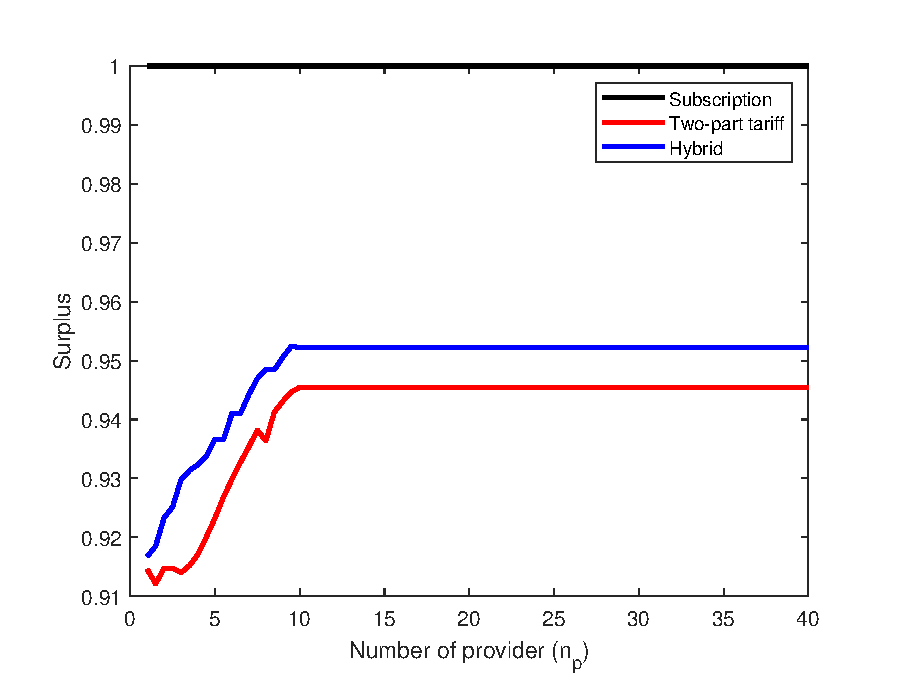
\includegraphics[width=8cm]{figure_3rd_final/f_low.eps} 
\textbf{\caption{Surplus Comparison for Extremely Low Operating Costs}}
\label{fig:app_lowxi}
\end{figure}

\subsection{Assumptions on Renters}
 
We conduct a numerical analysis for different shapes of the download frequency distribution. We vary the Pareto's shape parameter $b$ by three levels ($b=3, 4, \text{or } 5$) and present the results in \textbf{Figure \ref{fig:app_pareto}}. Here, the red (blue) line indicates the relative total surplus of the two-part tariff (the hybrid pricing) compared with the subscription-based pricing, which is represented as the horizontal black line. As suggested by our closed-form results, the total surplus of the two-part tariff and the hybrid pricing can be higher (lower) than the subscription-based pricing when the number of potential providers is small (large).

% \begin{figure}[ht!]
% \centering
% \includegraphics[width=8cm]{figure_3rd_final/f_main_modify.eps} 
% \caption{main}
% \end{figure}
%%%%%%%%%%%%%%%%%%%%%%%
\begin{figure}[ht!]
    \centering
    \subfigure[$b=3$]{\includegraphics[width=5cm]{figure_3rd_final/main_3.eps}}
    \subfigure[$b=4$]{\includegraphics[width=5cm]{figure_3rd_final/main_4.eps}}
    \subfigure[$b=5$]{\includegraphics[width=5cm]{figure_3rd_final/main_5.eps}}    
    \textbf{\caption{Numerical Analysis on Different Parameters of the Pareto Distribution.}}
    \label{fig:app_pareto}
\end{figure}

We examine whether the implications of pricing schemes are qualitatively consistent after relaxing this assumption that a renter's utility per bandwidth volume is independent of her download frequency. Specifically, we examine a scenario where potential renters with the higher utility per download volume tend to have more frequent download requests. We manipulate the shape parameter $b$ of the Pareto distribution---which determines the extent to which the bandwidth frequency is concentrated or dispersed---differently by the utility per bandwidth volume. We divide potential renters into two groups: 1) renters whose unit utility is uniformly distributed in $[0, 0.5]$ and whose frequency follows the Pareto distribution having a lighter tail (with $b_l=5$), and 2) those whose unit utility is uniformly distributed in $[0.5, 1]$ and whose frequency follows the Pareto distribution having a heavier tail (with $b_h=2$), where $b_l > b_h$. \textbf{Figure C.3} present the results for this scenario. The red (blue) line indicates the relative total surplus of the two-part tariff (the hybrid pricing) compared with the subscription-based pricing, which is represented as the horizontal black line. We observe that our main findings remain qualitatively consistent.

\begin{figure}[ht!]
\centering
\includegraphics[width=8cm]{figure_3rd_final/half_1.eps} 
\textbf{\caption{Numerical Analysis on Positive Association Between Utility per Download and Download Frequency}}
\label{fig:app_utilfreq}
\end{figure}

% R2's Points A2a (Renter's storage volume heterogeneity)
Lastly, we analyze the heterogeneity of storage demand. To do so, we redefine our utility functions to account for storage volume heterogeneity and determine renter parameters to explore.

\textbf{Generalized utility function.} Since the utility functions in our main model concern renters with a unit storage volume only, we need to define new utility functions for renters with heterogeneous storage volume. To do this, we have considered renter $i$ having storage volume $v_i$ and frequency $\lambda_i$. For this renter's utility function, we have assumed that 1) the benefit from P2P storage is proportional to $\lambda_i v_i$, 2) the storage cost is proportional to $v_i$, and 3) the bandwidth volume is $v_i$ times of the unit-volume renter with $\lambda_i$.

Based on these assumptions, we have seen that for the two-part tariff and subscription-based pricing, the new utility function is $v_i$ times of the previous function for a unit storage volume. However, the hybrid pricing might have various utility forms regarding how to price bandwidth services. For instance, the platform may offer the volume of bandwidth allowance proportionally to storage volume, which is widely observed in cloud service contracts. Also, the platform may provide the volume constantly across all renters regardless of their storage volume.

Since these possibilities seem plausible, we have examined both cases to explore the implications of hybrid pricing in the new setting. Below, we have specified the renter's utility functions in the current model and the extended ones that account for volume heterogeneity.

Here are the current utility functions of renters by pricing scheme:
\begin{equation*}
    U_i = \begin{cases}
    \lambda_i u_i - \theta p_s &\text{ under the subscription-based pricing,}\\
    \lambda_i u_i - \theta p_s - \max\{\lambda_i - q \lambda_0, 0\}p_b &\text{ under the hybrid pricing,}\\
    \lambda_i u_i - \theta p_s - \lambda_i p_b &\text{ under the two-part tariff.}
    \end{cases}
\end{equation*}
We generalize those functions for renter $i$'s storage volume $v_i$ as follows. First, when the bandwidth allowance is proportional to $v_i$, we can rewrite the functions as follows (\textbf{Utility Function I}):
\begin{equation*}
    U_i = \begin{cases}
    \lambda_i u_i v_i- \theta v_i p_s &\text{ under the subscription-based pricing,}\\
    \lambda_i u_i v_i- \theta v_i p_s - \max\{\lambda_i v_i - q \lambda_0 v_i, 0\}p_b &\text{ under the hybrid pricing,}\\
    \lambda_i u_i v_i- \theta v_i p_s - \lambda_i v_i p_b &\text{ under the two-part tariff.}
    \end{cases}
\end{equation*}
If $\lambda_0$ is independent of $v_i$, the utility is proportional to $v_i$ for all pricing schemes. Therefore, mere differences in storage demand do not affect a renter's adoption decision in this situation.

Second, we can rewrite the utility functions when the bandwidth allowance is constant as follows (\textbf{Utility Function II}): 
\begin{equation*}
    U_i = \begin{cases}
    \lambda_i u_i v_i- \theta v_i p_s &\text{ subscription}\\
    \lambda_i u_i v_i- \theta v_i p_s - \max\{\lambda_i v_i- q \lambda_0, 0\}p_b &\text{ hybrid}\\
    \lambda_i u_i v_i- \theta v_i p_s - \lambda_i v_i p_b &\text{ two-part tariff}
    \end{cases}
\end{equation*}
The notable difference is that the cost for bandwidth service in the hybrid pricing is not proportional to $v_i$. Specifically, the bandwidth fees are more burdensome for renters with high $v_i$ than those with low $v_i$. Noe that this situation is equivalent to having $v_i$ renters with a unit storage volume receives the free bandwidth allowance of $q\lambda_0 / v_i$. Therefore, the renter's decision can vary due to the storage demand.

\textbf{Renter heterogeneity.}  Considering the two types of possible utility functions, we conduct numerical studies on two renter-heterogeneity scenarios. First, we have examined the scenario where low-storage renters with storage volume ($v_l = 1$) and high-storage renters with storage volume ($v_h = 10$) have the same frequency distribution. We have set the parameters of Pareto distributions as $b_l = b_h = 2$ \textit{(\underline{Scenario i})}. Second, we have postulated that low-storage renters with storage volume ($v_l = 1$) and high-storage renters with storage volume ($v_h = 10$) have different frequency distributions. To make low-storage renters tend to request downloads more frequently than high-storage renters, we have chosen $b_l = 2$ and $b_h = 5$ for their Pareto distributions \textit{(\underline{Scenario ii})}.

To account for potential impacts of the renter composition, we have varied the proportions of low- and high-storage renters (9:1, 5:5, and 1:9) for each scenario. We have selected $q=3$ for our analysis. The results show that our findings remain consistent in all of the utility functions and scenarios (see \textbf{Figures C.4 through C.7}); that is, the total surplus of the two-part tariff (red lines) and that of the hybrid pricing (blue lines) can be higher/lower than the subscription-based pricing (normalized as 1, presented by the black horizontal line) when the number of potential providers is small/large. We find that the main insights from the basic setup remain qualitatively unchanged in our results.

%\textbf{Utility function I.} When the bandwidth allowance is proportional to a renter's storage volume

%\underline{\textit{Scenario i})} $(b_l, b_h) = (2, 2)$
%비중에 따른 3개 그래프\\
\begin{figure}[ht!]
    \centering
    \subfigure[$Low:High = 9:1$]{\includegraphics[width=5cm]{figure_3rd_final/prop_c_1.eps}}
    \subfigure[$Low:High = 5:5$]{\includegraphics[width=5cm]{figure_3rd_final/prop_c_2.eps}}
    \subfigure[$Low:High = 1:9$]{\includegraphics[width=5cm]{figure_3rd_final/prop_c_3.eps}}    
    \textbf{\caption{Numerical Analysis for Utility Function I and Scenario \textit{i}}}
\end{figure}\\

%\underline{\textit{Scenario ii})} $(b_l, b_h) = (2, 5)$
\begin{figure}[ht!]
    \centering
    \subfigure[$Low:High = 9:1$]{\includegraphics[width=5cm]{figure_3rd_final/prop_c_4_1.eps}}
    \subfigure[$Low:High = 5:5$]{\includegraphics[width=5cm]{figure_3rd_final/prop_c_5_1.eps}}
    \subfigure[$Low:High = 1:9$]{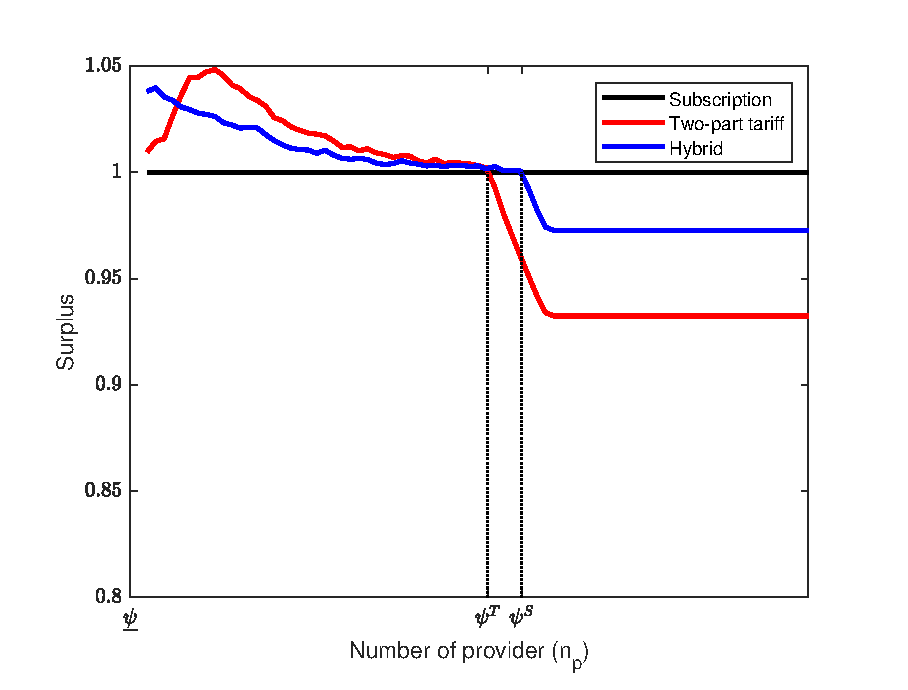
\includegraphics[width=5cm]{figure_3rd_final/prop_c_6_1.eps}}
    \textbf{\caption{Numerical Analysis for Utility Function I and Scenario \textit{ii}}}
\end{figure}
%- 아래의 pareto distribution에서 parameter가 달라질 때 효과와 연결\\
%- 용량이 큰 고객의 $b$가 큰 경우에, 이들에게는 i) first-best 인 부분에서 bandwidth에 비용을 지불받는 것의 merit이 줄어들어 subscription과 가까워짐 2) 마찬가지로 market-clearing에서도 bandwidth로부터 얻는 이익이 많이 없어져서 subscription과 가까워짐 -- c로 갈 수록 전체적으로 subscription과 가까워지는 모습(특히, hybrid)\\

%\textbf{Utility function II.}  When the bandwidth allowance is constant
\newpage
%\underline{\textit{Scenario i})} $(b_l, b_h) = (2, 2)$
\begin{figure}[ht!]
    \centering
    \subfigure[$Low:High = 9:1$]{\includegraphics[width=5cm]{figure_3rd_final/volume_c_1.eps}}
    \subfigure[$Low:High = 5:5$]{\includegraphics[width=5cm]{figure_3rd_final/volume_c_2.eps}}
    \subfigure[$Low:High = 1:9$]{\includegraphics[width=5cm]{figure_3rd_final/volume_c_3.eps}}
    \textbf{\caption{Numerical Analysis for Utility Function II and Scenario \textit{i}}}
\end{figure}

%\underline{\textit{Scenario ii})} $(b_l, b_h) = (2, 5)$
%%%%%%%%%%%%%%%%%%
\begin{figure}[ht!]
    \centering
    \subfigure[$Low:High = 9:1$]{\includegraphics[width=5cm]{figure_3rd_final/volume_c_4.eps}}
    \subfigure[$Low:High = 5:5$]{\includegraphics[width=5cm]{figure_3rd_final/volume_c_5.eps}}
    \subfigure[$Low:High = 1:9$]{\includegraphics[width=5cm]{figure_3rd_final/volume_c_6.eps}}
    \textbf{\caption{Numerical Analysis for Utility Function II and Scenario \textit{ii}}}
\end{figure}

\subsection{Hybrid Pricing and Profit Comparison}
In this numerical analysis, we compare a variety of $Hh$-type hybrid pricing schemes (i.e., $q>1$) with a two-part tariff and subscription-based pricing across different numbers of providers ($n_p$), redundancy rate ($\theta$) operating costs ($\xi$), and minimum download volumes ($\lambda_0$). Specifically, we consider the three following scenarios:

\begin{itemize}
    \item \textbf{Scenario 1: $(\theta, \xi, \lambda_0) = (2, 1.2, 2)$}
    \item \textbf{Scenario 2: $(\theta, \xi, \lambda_0) = (5, 1.2, 2)$}
    \item \textbf{Scenario 3: $(\theta, \xi, \lambda_0) = (2, 0.9, 1)$}
\end{itemize}

Note that we allow the number of providers ($n_p$) to change continuously within each scenario. Based on the parameter scenarios and the continuous $n_p$ region, we experiment with multiple values of free bandwidth allowance: 1 (or a two-part tariff), 1.05, 1.1., 2, 5, 10, 100, and $\infty$ (or subscription). In doing so, we fix $\alpha = 0.95$ and $n_r = 100$, and all parameter sets we consider here hold $\xi > \frac{3}{4}\alpha$.

\textbf{Figure C.8} shows the graphical results of our numerical analysis. On the left-hand side---i.e., \textbf{Figures C.8.}(a), (c), and (e), we present the absolute profit values by pricing scheme. We find that all these scenarios and $n_p$ regions show consistent patterns: the higher free bandwidth (i.e., higher $q$), the lower profit. As $q$ increases (from $q=1.05$ to $q=100$), the profit of hybrid pricing goes further away from that of the two-part tariff (line $T$) and approaches that of subscription-based pricing (line $S$).

Because the profit lines for the two-part tariff ($T$) and two small $q$'s ($q=1.05$ and $q=1.1$) overlap with each other on the profit plots, we zoom in on their relationships by plotting relative profits among these pricing schemes on the right-hand side---i.e., \textbf{Figures C.8.}(b), (d), and (f). Here, the vertical axis indicates the relative profits of hybrid pricing, which is each pricing scheme's profit divided by the two-part tariff's profit. We observe consistent patterns; that is, the higher $q$, the lower the relative profit.

% parameter sets:
% fixed : $\alpha = 0.95$, $n_r = 100$
% varied: $(\theta, \xi, \lambda_0) = (2, 1.2, 2)$, $(\theta, \xi, \lambda_0) = (5, 1.2, 2)$, $(\theta, \xi, \lambda_0) = (2, 0.9, 1)$
% Note., all parameter sets hold $\xi > \frac{3}{4}\alpha$.\\

\begin{figure}[ht!]
    \centering
    \subfigure[Profit (Scenario 1)]{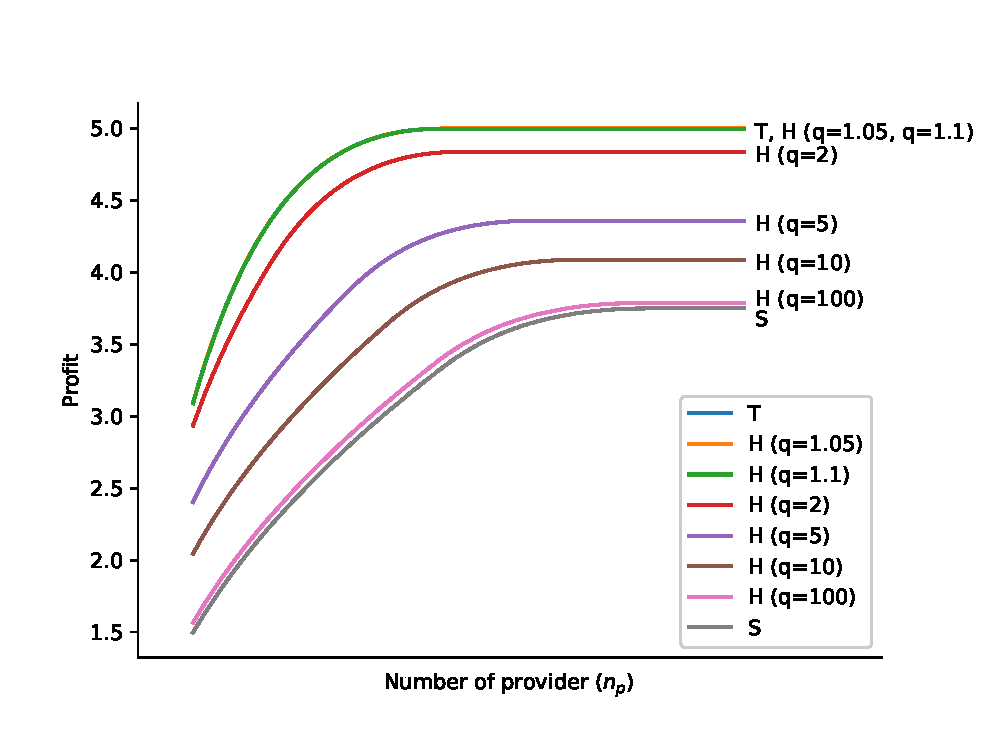
\includegraphics[width=7.5cm]{figure_3rd_final/p2pnum11.eps}}
    \subfigure[Relative profit (Scenario 1)]{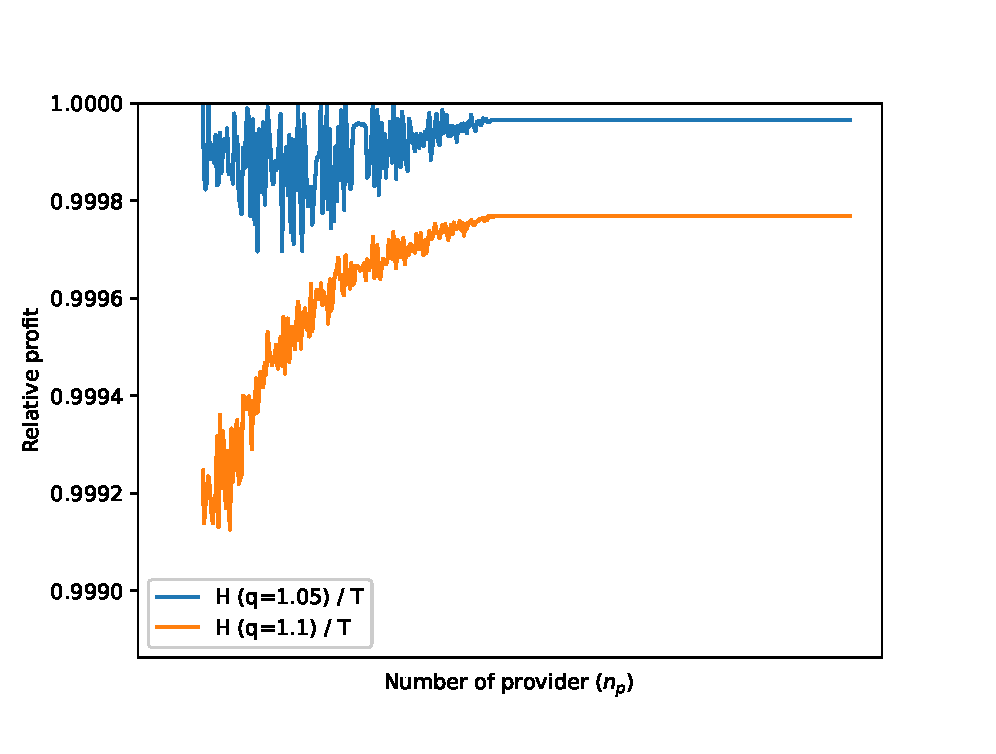
\includegraphics[width=7.5cm]{figure_3rd_final/p2pnum21.eps}}
    \subfigure[Profit (Scenario 2)]{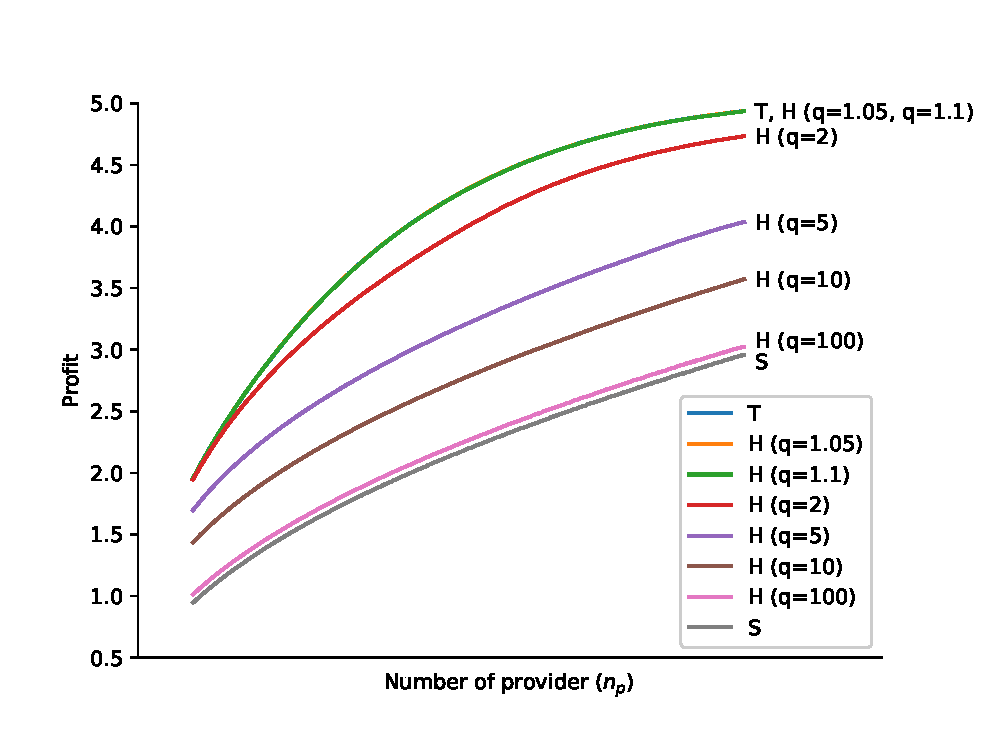
\includegraphics[width=7.5cm]{figure_3rd_final/p2pnum1a.eps}}
    \subfigure[Relative profit (Scenario 2)]{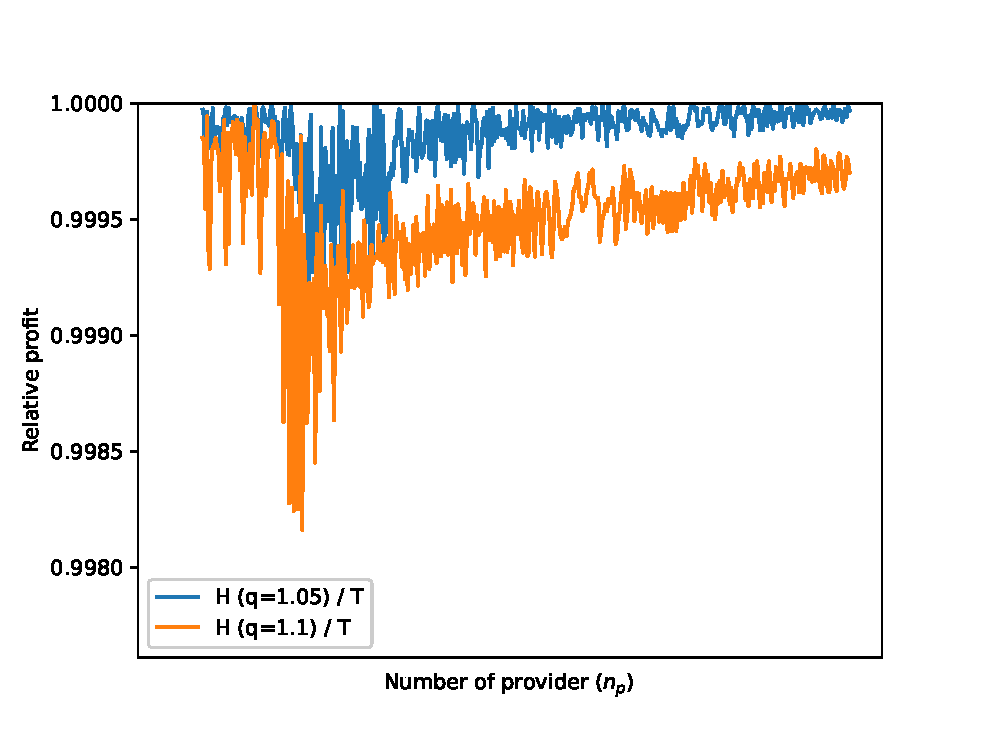
\includegraphics[width=7.5cm]{figure_3rd_final/p2pnum2a.eps}}
    \subfigure[Profit (Scenario 3)]{\includegraphics[width=7.5cm]{figure_3rd_final/p2pnum1b.eps}}
    \subfigure[Relative profit (Scenario 3)]{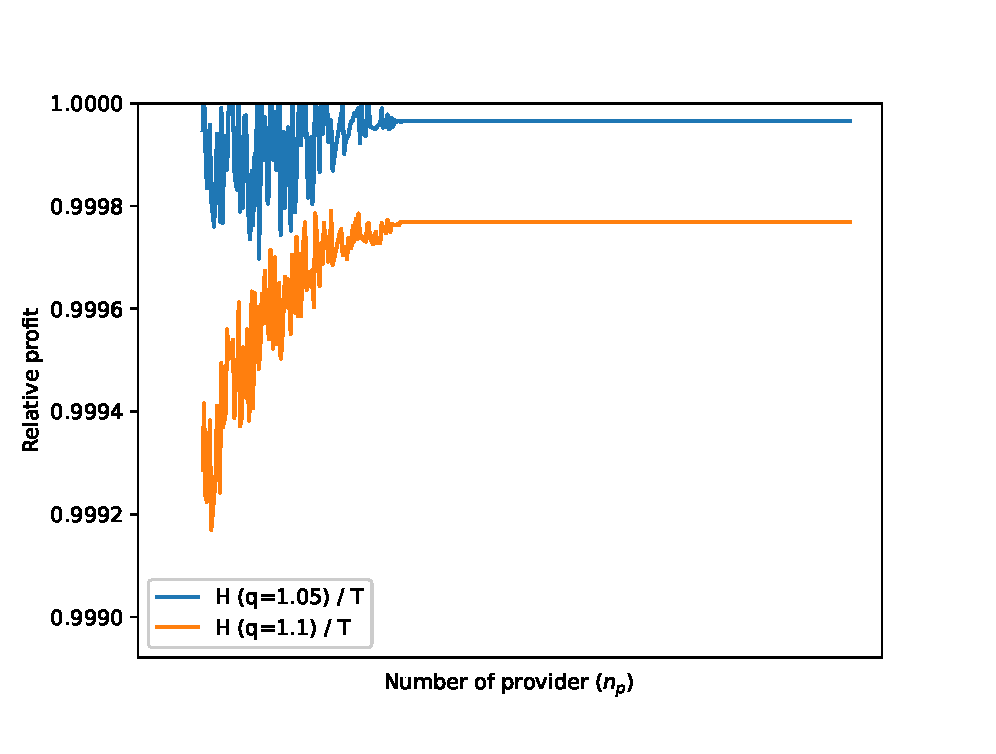
\includegraphics[width=7.5cm]{figure_3rd_final/p2pnum2b.eps}}
    \textbf{\caption{Numerical Analysis of Profit Comparison
}}
\end{figure}

\setlength{\baselineskip}{15pt}
	%\bibliographystyle{misqref}
    \bibliographystyle{informs2014}
	%\bibliographystyle{apacite}
	%\bibliographystyle{pomsref}
	\bibliography{bib}

\end{document}